\documentclass[openany]{article}
\usepackage{lmodern}
\usepackage{amssymb,amsmath}
\usepackage{ifxetex,ifluatex}
\usepackage{fixltx2e} % provides \textsubscript
\ifnum 0\ifxetex 1\fi\ifluatex 1\fi=0 % if pdftex
  \usepackage[T1]{fontenc}
  \usepackage[utf8]{inputenc}
\else % if luatex or xelatex
  \ifxetex
    \usepackage{mathspec}
  \else
    \usepackage{fontspec}
  \fi
  \defaultfontfeatures{Ligatures=TeX,Scale=MatchLowercase}
\fi
% use upquote if available, for straight quotes in verbatim environments
\IfFileExists{upquote.sty}{\usepackage{upquote}}{}
% use microtype if available
\IfFileExists{microtype.sty}{%
\usepackage{microtype}
\UseMicrotypeSet[protrusion]{basicmath} % disable protrusion for tt fonts
}{}
\usepackage{hyperref}
\PassOptionsToPackage{usenames,dvipsnames}{color} % color is loaded by hyperref
\hypersetup{unicode=true,
            pdftitle={Informatics team manual of procedures},
            pdfauthor={Ania Tassinari \& Caitlin Guccione},
            colorlinks=true,
            linkcolor=Maroon,
            citecolor=Blue,
            urlcolor=blue,
            breaklinks=true}
\urlstyle{same}  % don't use monospace font for urls
\usepackage{natbib}
\bibliographystyle{apalike}
\usepackage{color}
\usepackage{fancyvrb}
\newcommand{\VerbBar}{|}
\newcommand{\VERB}{\Verb[commandchars=\\\{\}]}
\DefineVerbatimEnvironment{Highlighting}{Verbatim}{commandchars=\\\{\}}
% Add ',fontsize=\small' for more characters per line
\usepackage{framed}
\definecolor{shadecolor}{RGB}{248,248,248}
\newenvironment{Shaded}{\begin{snugshade}}{\end{snugshade}}
\newcommand{\AlertTok}[1]{\textcolor[rgb]{0.94,0.16,0.16}{#1}}
\newcommand{\AnnotationTok}[1]{\textcolor[rgb]{0.56,0.35,0.01}{\textbf{\textit{#1}}}}
\newcommand{\AttributeTok}[1]{\textcolor[rgb]{0.77,0.63,0.00}{#1}}
\newcommand{\BaseNTok}[1]{\textcolor[rgb]{0.00,0.00,0.81}{#1}}
\newcommand{\BuiltInTok}[1]{#1}
\newcommand{\CharTok}[1]{\textcolor[rgb]{0.31,0.60,0.02}{#1}}
\newcommand{\CommentTok}[1]{\textcolor[rgb]{0.56,0.35,0.01}{\textit{#1}}}
\newcommand{\CommentVarTok}[1]{\textcolor[rgb]{0.56,0.35,0.01}{\textbf{\textit{#1}}}}
\newcommand{\ConstantTok}[1]{\textcolor[rgb]{0.00,0.00,0.00}{#1}}
\newcommand{\ControlFlowTok}[1]{\textcolor[rgb]{0.13,0.29,0.53}{\textbf{#1}}}
\newcommand{\DataTypeTok}[1]{\textcolor[rgb]{0.13,0.29,0.53}{#1}}
\newcommand{\DecValTok}[1]{\textcolor[rgb]{0.00,0.00,0.81}{#1}}
\newcommand{\DocumentationTok}[1]{\textcolor[rgb]{0.56,0.35,0.01}{\textbf{\textit{#1}}}}
\newcommand{\ErrorTok}[1]{\textcolor[rgb]{0.64,0.00,0.00}{\textbf{#1}}}
\newcommand{\ExtensionTok}[1]{#1}
\newcommand{\FloatTok}[1]{\textcolor[rgb]{0.00,0.00,0.81}{#1}}
\newcommand{\FunctionTok}[1]{\textcolor[rgb]{0.00,0.00,0.00}{#1}}
\newcommand{\ImportTok}[1]{#1}
\newcommand{\InformationTok}[1]{\textcolor[rgb]{0.56,0.35,0.01}{\textbf{\textit{#1}}}}
\newcommand{\KeywordTok}[1]{\textcolor[rgb]{0.13,0.29,0.53}{\textbf{#1}}}
\newcommand{\NormalTok}[1]{#1}
\newcommand{\OperatorTok}[1]{\textcolor[rgb]{0.81,0.36,0.00}{\textbf{#1}}}
\newcommand{\OtherTok}[1]{\textcolor[rgb]{0.56,0.35,0.01}{#1}}
\newcommand{\PreprocessorTok}[1]{\textcolor[rgb]{0.56,0.35,0.01}{\textit{#1}}}
\newcommand{\RegionMarkerTok}[1]{#1}
\newcommand{\SpecialCharTok}[1]{\textcolor[rgb]{0.00,0.00,0.00}{#1}}
\newcommand{\SpecialStringTok}[1]{\textcolor[rgb]{0.31,0.60,0.02}{#1}}
\newcommand{\StringTok}[1]{\textcolor[rgb]{0.31,0.60,0.02}{#1}}
\newcommand{\VariableTok}[1]{\textcolor[rgb]{0.00,0.00,0.00}{#1}}
\newcommand{\VerbatimStringTok}[1]{\textcolor[rgb]{0.31,0.60,0.02}{#1}}
\newcommand{\WarningTok}[1]{\textcolor[rgb]{0.56,0.35,0.01}{\textbf{\textit{#1}}}}
\usepackage{longtable,booktabs}
\usepackage{graphicx,grffile}
\makeatletter
\def\maxwidth{\ifdim\Gin@nat@width>\linewidth\linewidth\else\Gin@nat@width\fi}
\def\maxheight{\ifdim\Gin@nat@height>\textheight\textheight\else\Gin@nat@height\fi}
\makeatother
% Scale images if necessary, so that they will not overflow the page
% margins by default, and it is still possible to overwrite the defaults
% using explicit options in \includegraphics[width, height, ...]{}
\setkeys{Gin}{width=\maxwidth,height=\maxheight,keepaspectratio}
\IfFileExists{parskip.sty}{%
\usepackage{parskip}
}{% else
\setlength{\parindent}{0pt}
\setlength{\parskip}{6pt plus 2pt minus 1pt}
}
\setlength{\emergencystretch}{3em}  % prevent overfull lines
\providecommand{\tightlist}{%
  \setlength{\itemsep}{0pt}\setlength{\parskip}{0pt}}
\setcounter{secnumdepth}{5}
% Redefines (sub)paragraphs to behave more like sections
\ifx\paragraph\undefined\else
\let\oldparagraph\paragraph
\renewcommand{\paragraph}[1]{\oldparagraph{#1}\mbox{}}
\fi
\ifx\subparagraph\undefined\else
\let\oldsubparagraph\subparagraph
\renewcommand{\subparagraph}[1]{\oldsubparagraph{#1}\mbox{}}
\fi

%%% Use protect on footnotes to avoid problems with footnotes in titles
\let\rmarkdownfootnote\footnote%
\def\footnote{\protect\rmarkdownfootnote}

%%% Change title format to be more compact
\usepackage{titling}

% Create subtitle command for use in maketitle
\providecommand{\subtitle}[1]{
  \posttitle{
    \begin{center}\large#1\end{center}
    }
}

\setlength{\droptitle}{-2em}

  \title{Informatics team manual of procedures}
    \pretitle{\vspace{\droptitle}\centering\huge}
  \posttitle{\par}
    \author{Ania Tassinari \& Caitlin Guccione}
    \preauthor{\centering\large\emph}
  \postauthor{\par}
      \predate{\centering\large\emph}
  \postdate{\par}
    \date{2019-07-12}

\usepackage{booktabs}
\usepackage{amsthm}
\makeatletter
\def\thm@space@setup{%
  \thm@preskip=8pt plus 2pt minus 4pt
  \thm@postskip=\thm@preskip
}
\makeatother

\begin{document}
\maketitle

{
\hypersetup{linkcolor=black}
\setcounter{tocdepth}{2}
\tableofcontents
}
\hypertarget{about}{%
\section{About}\label{about}}

This is a manual of operations for the Agios Informatics team. Its puspose is to:

\begin{itemize}
\tightlist
\item
  provide a resource on \textbf{best practices} (\ref{bestpractices})
\item
  aid in setting up effective and reproducible \textbf{project workflows} (\ref{workflows})
\item
  promote learning and sharing of \textbf{ideas} (\ref{toolbox}).
\end{itemize}

\hypertarget{bestpractices}{%
\section{Best practices}\label{bestpractices}}

\hypertarget{reproducible-research}{%
\subsection{Reproducible research}\label{reproducible-research}}

\hypertarget{purpose}{%
\subsubsection{Purpose}\label{purpose}}

\begin{enumerate}
\def\labelenumi{\arabic{enumi}.}
\tightlist
\item
  Improve collaborative analyses:
\end{enumerate}

\begin{itemize}
\tightlist
\item
  make sharing easier
\item
  enable retrieval and interpretation of results long after analysis ended
\end{itemize}

\begin{enumerate}
\def\labelenumi{\arabic{enumi}.}
\setcounter{enumi}{1}
\item
  Simplify hand-off to Biostats
\item
  Improve confidence in our data and results
\end{enumerate}

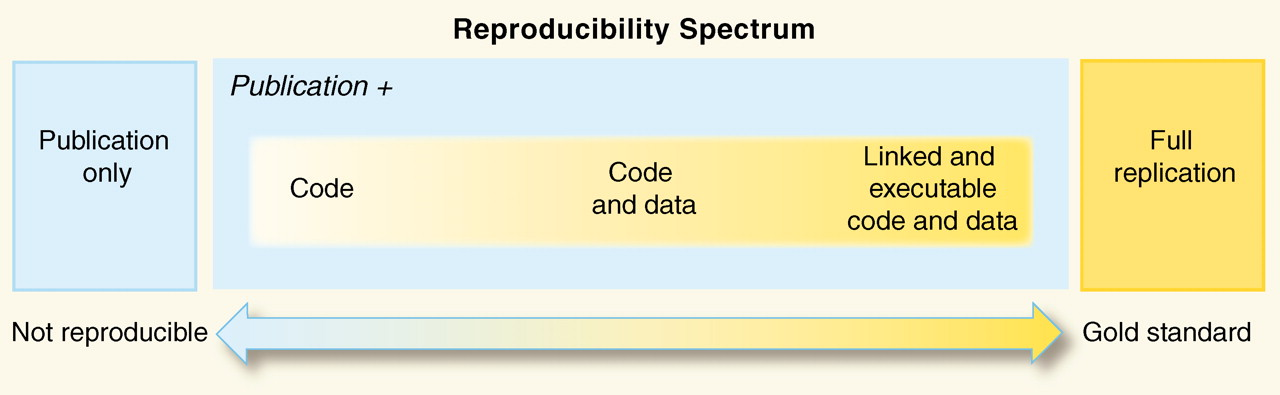
\includegraphics{images/reprodresearch.jpg}

Source: Peng et al., \emph{Reproducible Research in Computational Science}. Science 2011.

\hypertarget{dos-and-donts-of-reproducible-research}{%
\subsubsection{DO's and DON'T's of reproducible research}\label{dos-and-donts-of-reproducible-research}}

\begin{itemize}
\tightlist
\item
  DO start with good science
\item
  DON'T do things by hand

  \begin{itemize}
  \tightlist
  \item
    Was any part of this analysis done by hand?

    \begin{itemize}
    \tightlist
    \item
      If so, are those parts precisely documented?
    \item
      Does the documentation match reality?
    \end{itemize}
  \end{itemize}
\item
  DON'T point and click
\item
  DO teach a computer
\item
  DO use version control
\item
  DO keep track of your software environment
\item
  DON'T save any output (until it's time to write a paper)
\item
  DO set your seed
\end{itemize}

Source: Reproducible Research at Coursera

\hypertarget{version-control}{%
\subsection{Version control}\label{version-control}}

\hypertarget{code-guidelines}{%
\subsection{Code guidelines}\label{code-guidelines}}

\hypertarget{r}{%
\subsubsection{R}\label{r}}

\begin{itemize}
\tightlist
\item
  \href{https://style.tidyverse.org}{Tidyverse Style Guide}
\item
  \href{https://google.github.io/styleguide/Rguide.xml}{Google's R Style Guide}
\end{itemize}

\hypertarget{workflows}{%
\section{Project Workflows}\label{workflows}}

\hypertarget{using-workflowr}{%
\subsection{Using Workflowr}\label{using-workflowr}}

\hypertarget{quick-start}{%
\subsubsection{Quick Start}\label{quick-start}}

This section is a quick version setting up workflowr, for more clear or specific instructions skip to \protect\hyperlink{the-full-guide-to-using-workflowr}{The Full Guide to Using Workflowr}.

\hypertarget{set-up}{%
\paragraph{Set Up}\label{set-up}}

In the \texttt{Console} tab of RStudio make sure you are in \texttt{(None)} project:

\begin{Shaded}
\begin{Highlighting}[]
\KeywordTok{install.packages}\NormalTok{(}\StringTok{"workflowr"}\NormalTok{)}
\KeywordTok{library}\NormalTok{(}\StringTok{"workflowr"}\NormalTok{)}
\KeywordTok{wflow_git_config}\NormalTok{(}\DataTypeTok{user.name =} \StringTok{"First Last"}\NormalTok{, }
    \DataTypeTok{user.email =} \StringTok{"first.last@agios.com"}\NormalTok{)}
\end{Highlighting}
\end{Shaded}

\protect\hyperlink{installation}{Click here for more specfic details on \textbf{set up}}

\hypertarget{creating-projects}{%
\paragraph{Creating Projects}\label{creating-projects}}

In the \texttt{Console} tab,

\begin{Shaded}
\begin{Highlighting}[]
\KeywordTok{wflow_start}\NormalTok{(}\StringTok{"PROJECT_NAME"}\NormalTok{)}
\KeywordTok{wflow_build}\NormalTok{()}
\KeywordTok{wflow_publish}\NormalTok{(}\KeywordTok{c}\NormalTok{(}\StringTok{"analysis/*.Rmd"}\NormalTok{), }
    \StringTok{"Publish the initial files for PROJECT_NAME"}\NormalTok{)}
\end{Highlighting}
\end{Shaded}

\protect\hyperlink{create-project}{Click here for more specfic details on \textbf{creating projects}}

\hypertarget{connecting-to-gitlab}{%
\paragraph{Connecting to GitLab}\label{connecting-to-gitlab}}

In the \texttt{Console} tab,

\begin{Shaded}
\begin{Highlighting}[]
\KeywordTok{wflow_use_gitlab}\NormalTok{(}\DataTypeTok{username =} \StringTok{"first.last"}\NormalTok{, }
    \DataTypeTok{repository =} \StringTok{"PROJECT_NAME"}\NormalTok{, }
    \DataTypeTok{domain =} \StringTok{"ceres.agios.com"}\NormalTok{)}
\end{Highlighting}
\end{Shaded}

Go to your Agios GitLab and do the following:

\begin{itemize}
\tightlist
\item
  Create a project in GitLab with the same name as the project in RStudio

  \begin{itemize}
  \tightlist
  \item
    We called our project: PROJECT\_NAME
  \end{itemize}
\item
  Scroll down to the push an existing Git repository option

  \begin{itemize}
  \tightlist
  \item
    Copy everything in the box besides the first line (\texttt{cd\ existing\_repo})
  \end{itemize}
\item
  Make sure you are in PROJECT\_NAME directory

  \begin{itemize}
  \tightlist
  \item
    Paste what you just copied from Git into the \texttt{Terminal} tab in RStudio
  \end{itemize}
\end{itemize}

\protect\hyperlink{connecting-to-gitlab-1}{Click here for more specfic details on connecting to \textbf{GitLab}}

\hypertarget{creating-a-new-file}{%
\paragraph{Creating a New File}\label{creating-a-new-file}}

In the \texttt{Console} tab,

\begin{Shaded}
\begin{Highlighting}[]
\KeywordTok{wflow_open}\NormalTok{(}\StringTok{"analysis/NEW_FILE.Rmd"}\NormalTok{)}
\KeywordTok{wflow_build}\NormalTok{()}
\KeywordTok{wflow_publish}\NormalTok{(}\KeywordTok{c}\NormalTok{(}\StringTok{"analysis/*.Rmd"}\NormalTok{), }
    \StringTok{"Publish the file NEW_FILE"}\NormalTok{)}
\end{Highlighting}
\end{Shaded}

In the \texttt{Terminal} tab,

\begin{Shaded}
\begin{Highlighting}[]
\NormalTok{git push}
\end{Highlighting}
\end{Shaded}

\protect\hyperlink{adding-new-files}{Click here for more specfic details on \textbf{creating new files}}

\begin{center}\includegraphics[width=0.7\linewidth]{images/Workflow_Photos/uMadeIt2} \end{center}

\hypertarget{quick-useful-additions}{%
\paragraph{Quick Useful Additions}\label{quick-useful-additions}}

\hypertarget{adding-packrat}{%
\paragraph{Adding PackRat}\label{adding-packrat}}

PackRat records or saves the exact package versions that you depend on and stores them in GitLab.

\begin{enumerate}
\def\labelenumi{\arabic{enumi}.}
\tightlist
\item
  Install PackRat
\end{enumerate}

\begin{Shaded}
\begin{Highlighting}[]
\KeywordTok{install.packages}\NormalTok{(}\StringTok{"packrat"}\NormalTok{)}
\end{Highlighting}
\end{Shaded}

\begin{enumerate}
\def\labelenumi{\arabic{enumi}.}
\setcounter{enumi}{1}
\item
  Add PackRat to Existing Project

  \begin{itemize}
  \tightlist
  \item
    Go to \texttt{Tools}
  \item
    Click on \texttt{Project\ Options}
  \item
    Click \texttt{Add\ PackRat} then check \texttt{Use\ PackRat\ for\ this\ project}
  \item
    Now, check the following boxes (shown in the image below) and tap \texttt{OK} *:
  \end{itemize}
\end{enumerate}

\begin{itemize}
\tightlist
\item
  This step may take a while if you have a number of packages you are backing up.
\end{itemize}

\begin{figure}

{\centering \includegraphics[width=0.6\linewidth]{images/Workflow_Photos/packRat} 

}

\caption{Showing how to install PackRat into a current project with the suggested selections}\label{fig:c999}
\end{figure}

\protect\hyperlink{adding-packrat-1}{Click here for more specfic details on \textbf{PackRat}}

\hypertarget{update-session-information-function}{%
\subparagraph{Update Session Information Function}\label{update-session-information-function}}

Add the following line to your \texttt{\_workflowr.yml} file :

\begin{Shaded}
\begin{Highlighting}[]
\NormalTok{sessioninfo}\OperatorTok{:}\StringTok{"devtools::session_info()"}
\end{Highlighting}
\end{Shaded}

\protect\hyperlink{update-session-information-function-1}{Click here for more specfic details on \textbf{Session Info}}

\hypertarget{publish-to-gitlab-without-rebuilding-sites}{%
\subparagraph{Publish to GitLab without Rebuilding Sites}\label{publish-to-gitlab-without-rebuilding-sites}}

A quicker way to push to GitLab without rebuilding your website.

\begin{enumerate}
\def\labelenumi{\arabic{enumi}.}
\tightlist
\item
  Edit the Rmd file and save your changes
\item
  Run one of the following commands (doesn't matter which one you select)

  \begin{itemize}
  \tightlist
  \item
    \texttt{wflow\_build()}

    \begin{itemize}
    \tightlist
    \item
      It doesn't matter if we build other files, they won't be added to git unless we add them in the next step
    \end{itemize}
  \item
    \texttt{wflow\_build("file.rmd")}
  \item
    Knit the file
  \end{itemize}
\item
  \texttt{wflow\_git\_commit("file.rmd",\ "This\ is\ your\ commit\ message")}
\item
  Flip into the terminal and run \texttt{git\ push()}
\end{enumerate}

\begin{center}\rule{0.5\linewidth}{\linethickness}\end{center}

\hypertarget{the-full-guide-to-using-workflowr}{%
\subsubsection*{The Full Guide to Using Workflowr}\label{the-full-guide-to-using-workflowr}}
\addcontentsline{toc}{subsubsection}{The Full Guide to Using Workflowr}

\hypertarget{installation}{%
\subsubsection{Installation}\label{installation}}

\hypertarget{programs-needed}{%
\paragraph{Programs Needed}\label{programs-needed}}

We are assuming that you already have RStuido and GitLab, for this implementation we are using the RStudio on the new server (hpc.agios.local) which is RStudio version 1.2.1335.1.

If you don't have GitLab you need to have an account set up through Agios. If you don't have the updated RStudio you need to get access to the new server and then use the following link : \href{https://hpc.agios.local}{hpc.agios.local}

\hypertarget{installing-workflowr}{%
\paragraph{Installing Workflowr}\label{installing-workflowr}}

\begin{enumerate}
\def\labelenumi{\arabic{enumi}.}
\tightlist
\item
  Open RStudio and change project in the top right corner to \texttt{(None)}

  \begin{itemize}
  \tightlist
  \item
    Make sure you are in your home directory on RStudio as well, thus in the bottom right corner of your screen under \texttt{New\ Folder}, it is labeled \texttt{Home} with a small house.
  \end{itemize}
\item
  In the \texttt{Console} tab located in the bottom left hand corner type:
\end{enumerate}

\begin{Shaded}
\begin{Highlighting}[]
\KeywordTok{install.packages}\NormalTok{(}\StringTok{"workflowr"}\NormalTok{)}
\end{Highlighting}
\end{Shaded}

\begin{enumerate}
\def\labelenumi{\arabic{enumi}.}
\setcounter{enumi}{2}
\tightlist
\item
  Confirm you have access to Workflowr, in the \texttt{Console} tab:
\end{enumerate}

\begin{Shaded}
\begin{Highlighting}[]
\KeywordTok{library}\NormalTok{(}\StringTok{"workflowr"}\NormalTok{)}
\end{Highlighting}
\end{Shaded}

\hypertarget{configure-git-this-only-needs-to-be-done-once-per-laptop}{%
\paragraph{\texorpdfstring{Configure Git\emph{
}This only needs to be done once per laptop}{Configure Git This only needs to be done once per laptop}}\label{configure-git-this-only-needs-to-be-done-once-per-laptop}}

In the \texttt{Console} tab:

\begin{Shaded}
\begin{Highlighting}[]
\KeywordTok{wflow_git_config}\NormalTok{(}\DataTypeTok{user.name =} \StringTok{"First Last"}\NormalTok{, }
    \DataTypeTok{user.email =} \StringTok{"first.last@agios.com"}\NormalTok{)}
\end{Highlighting}
\end{Shaded}

\hypertarget{create-project}{%
\subsubsection{Create Project}\label{create-project}}

\hypertarget{start-project}{%
\paragraph{Start Project}\label{start-project}}

In the \texttt{Console} tab:

\begin{Shaded}
\begin{Highlighting}[]
\KeywordTok{wflow_start}\NormalTok{(}\StringTok{"PROJECT_NAME"}\NormalTok{)}
\end{Highlighting}
\end{Shaded}

\begin{enumerate}
\def\labelenumi{\arabic{enumi}.}
\tightlist
\item
  What does \texttt{wflow\_start} do?

  \begin{itemize}
  \tightlist
  \item
    Creates a directory that contains all files necessary to start a workflowr project
  \item
    Changes your current directory to PROJECT\_NAME
  \item
    Creates a \texttt{.git} folder which we will connect to GitLab repository
  \end{itemize}
\item
  What is the \texttt{analysis} folder for?

  \begin{itemize}
  \tightlist
  \item
    Contains all source R Markdown files (Rmd)

    \begin{itemize}
    \tightlist
    \item
      Includes: \texttt{index.rmd}*

      \begin{itemize}
      \tightlist
      \item
        Contains no R code but generates \texttt{index.html} which eventually runs the entire project
      \end{itemize}
    \end{itemize}
  \item
    Contains \texttt{\_site.yml}

    \begin{itemize}
    \tightlist
    \item
      Allows user to edit theme, navigation bar, menus ect.
    \item
      Helpful \href{https://bookdown.org/yihui/rmarkdown/rmarkdown-site.html}{link} to customizing
    \end{itemize}
  \end{itemize}
\item
  What is the \texttt{docs} folder for?

  \begin{itemize}
  \tightlist
  \item
    Contains all HTML files for webpage

    \begin{itemize}
    \tightlist
    \item
      Note that this file will be empty until we build the project
    \item
      Each HTML file is built from a corresponding Rmd file in the \texttt{analysis} folder
    \end{itemize}
  \item
    Contains any figures created by Rmd files
  \end{itemize}
\item
  What about the \texttt{data}, \texttt{code} and \texttt{output} files?

  \begin{itemize}
  \tightlist
  \item
    These files are there for your use and thus can be deleted if desired
  \end{itemize}
\end{enumerate}

\hypertarget{build-project}{%
\paragraph{Build Project*}\label{build-project}}

In the \texttt{Console} tab:

\begin{Shaded}
\begin{Highlighting}[]
\KeywordTok{wflow_build}\NormalTok{()}
\end{Highlighting}
\end{Shaded}

\begin{enumerate}
\def\labelenumi{\arabic{enumi}.}
\tightlist
\item
  What does \texttt{wflow\_build()} do?

  \begin{itemize}
  \tightlist
  \item
    Builds all the R Markdown files in analysis and saves their HTML in docs
  \item
    Displays the website
  \end{itemize}
\end{enumerate}

Your website should be similar to the image of mine shown below (except with a Publish tab instead of a Dates tab)

\begin{figure}

{\centering 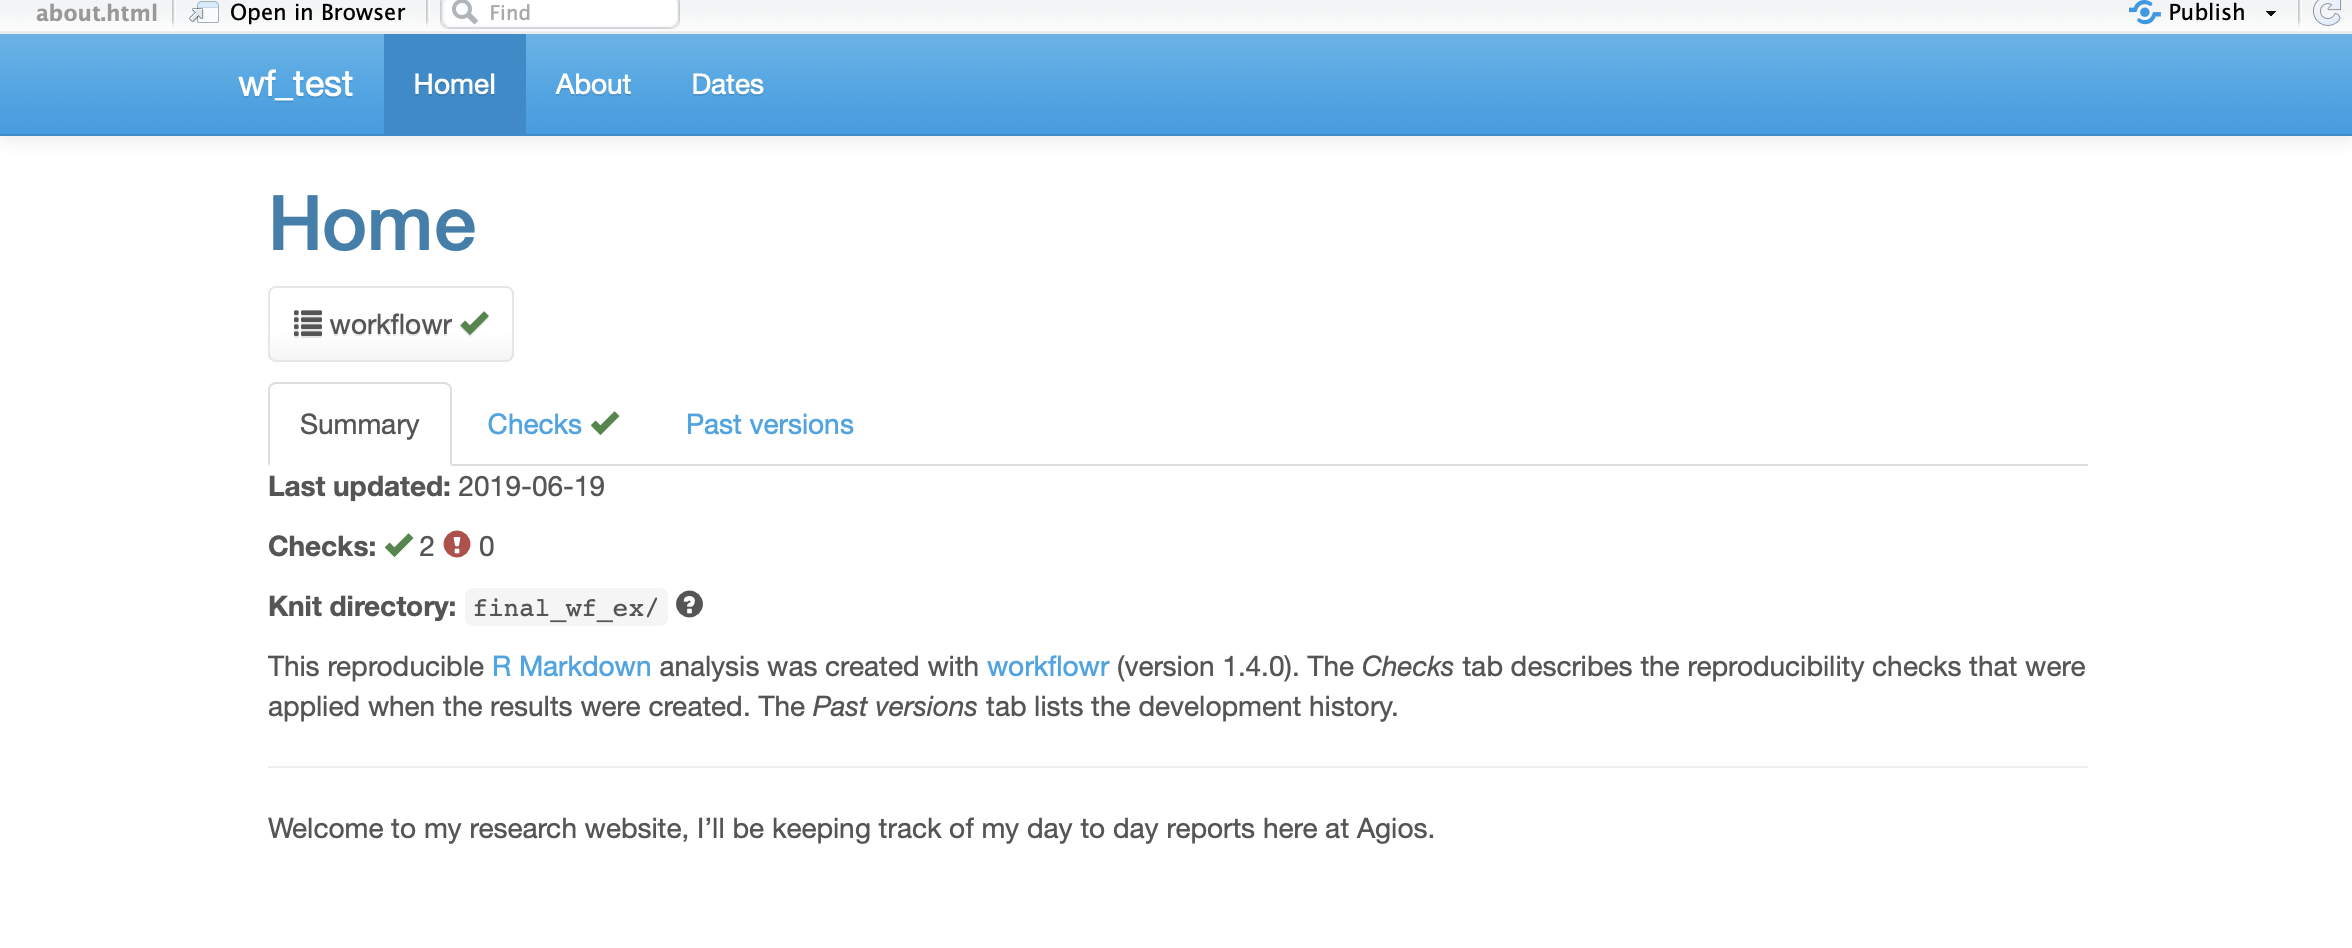
\includegraphics[width=0.9\linewidth]{images/Workflow_Photos/sample_wf} 

}

\caption{An example of a sucessfully built workflowr page}\label{fig:c4}
\end{figure}

\hypertarget{view-project}{%
\paragraph{View Project*}\label{view-project}}

At any time you can view the current site on your local machine by typing in the \texttt{Console} tab:

\begin{Shaded}
\begin{Highlighting}[]
\KeywordTok{wflow_view}\NormalTok{()}
\end{Highlighting}
\end{Shaded}

*Shortcut : You can use the knit button to do both of these

\hypertarget{publish-website}{%
\paragraph{Publish Website}\label{publish-website}}

Currently, our project is simply an HTML file stored on our laptop, publishing the website will make it available online.

In the \texttt{Console} tab:

\begin{Shaded}
\begin{Highlighting}[]
\KeywordTok{wflow_status}\NormalTok{()}
\end{Highlighting}
\end{Shaded}

This allows you to view which files are published or unpublished currently.

Now we want to publish our page the command to do so takes three parts

\begin{enumerate}
\def\labelenumi{\arabic{enumi}.}
\tightlist
\item
  c - Stands for commit
\item
  (``analysis/index.Rmd'', ``analysis/about.Rmd'', ``analysis/license.Rmd'')

  \begin{itemize}
  \tightlist
  \item
    A character vector of the Rmd files you want to be published
  \item
    It may be easier to place ("*.Rmd") here to use all the files
  \end{itemize}
\item
  ``Publish the initial files for PROJECT\_NAME'' - A commit message to be posted
\end{enumerate}

Overall, \texttt{wflow\_publish} is a quick and error-free way for us to commit and push all of our Rmd files to our GitLab at once.

In the \texttt{Console} tab:

\begin{Shaded}
\begin{Highlighting}[]
\KeywordTok{wflow_publish}\NormalTok{(}\KeywordTok{c}\NormalTok{(}\StringTok{"analysis/index.Rmd"}\NormalTok{, }
    \StringTok{"analysis/about.Rmd"}\NormalTok{, }\StringTok{"analysis/license.Rmd"}\NormalTok{), }
    \StringTok{"Publish the initial files for PROJECT_NAME"}\NormalTok{)}
\end{Highlighting}
\end{Shaded}

\hypertarget{connecting-to-gitlab-1}{%
\subsubsection{Connecting to GitLab}\label{connecting-to-gitlab-1}}

\hypertarget{creating-a-remote-repository-on-gitlab}{%
\paragraph{Creating a remote repository on GitLab}\label{creating-a-remote-repository-on-gitlab}}

\begin{enumerate}
\def\labelenumi{\arabic{enumi}.}
\tightlist
\item
  Log in to GitLab and click \texttt{New\ Project}
\item
  The project name in GitLab has to be the same name as the project name in RStudio: PROJECT\_NAME
\item
  Make sure to save it as \texttt{Internal} so everyone at Agios can see it
\end{enumerate}

\hypertarget{not-working-do-you-have-an-ssh-key}{%
\paragraph{Not working? Do you have an ssh key? *}\label{not-working-do-you-have-an-ssh-key}}
\addcontentsline{toc}{paragraph}{Not working? Do you have an ssh key? *}

In order for you to successfully connect to GitLab, you need to have an ssh key linked to your GitLab.

There is a simple guide to doing this on GitLab \href{http://ceres.agios.com/help/ssh/README\#generating-a-new-ssh-key-pair}{here} so you can simply follow along below and click the link if you get lost.

\begin{enumerate}
\def\labelenumi{\arabic{enumi}.}
\tightlist
\item
  Automatically copy your public key to the clipboard using one of the following commands:
\end{enumerate}

\begin{Shaded}
\begin{Highlighting}[]
\CommentTok{# macOS:}
\ExtensionTok{pbcopy} \OperatorTok{<}\NormalTok{ ~/.ssh/id_ed25519.pub}
\CommentTok{# WSL / GNU/Linux (requires the xclip package):}
\ExtensionTok{xclip}\NormalTok{ -sel clip }\OperatorTok{<}\NormalTok{ ~/.ssh/id_ed25519.pub}
\CommentTok{#Git Bash on Windows:}
\FunctionTok{cat}\NormalTok{ ~/.ssh/id_ed25519.pub }\KeywordTok{|} \ExtensionTok{clip}
\end{Highlighting}
\end{Shaded}

\begin{enumerate}
\def\labelenumi{\arabic{enumi}.}
\setcounter{enumi}{1}
\tightlist
\item
  Go back into your GitLab account and click on \texttt{Settings} then \texttt{SSH\ Keys} and simply paste there.
\end{enumerate}

\begin{itemize}
\tightlist
\item
  Only need to do this once per laptop or GitLab account
\end{itemize}

\hypertarget{connect-rstudio-and-gitlab}{%
\paragraph{Connect RStudio and GitLab}\label{connect-rstudio-and-gitlab}}

\begin{enumerate}
\def\labelenumi{\arabic{enumi}.}
\tightlist
\item
  Go to RStudio, in \texttt{Console} tab, type:
\end{enumerate}

\begin{Shaded}
\begin{Highlighting}[]
\KeywordTok{wflow_use_gitlab}\NormalTok{(}\DataTypeTok{username =} \StringTok{"first.last"}\NormalTok{, }
    \DataTypeTok{repository =} \StringTok{"PROJECT_NAME"}\NormalTok{, }
    \DataTypeTok{domain =} \StringTok{"ceres.agios.com"}\NormalTok{)}
\end{Highlighting}
\end{Shaded}

\begin{enumerate}
\def\labelenumi{\arabic{enumi}.}
\setcounter{enumi}{1}
\tightlist
\item
  Go back to GitLab and scroll down to the \texttt{push\ an\ existing\ Git\ repository} option

  \begin{itemize}
  \tightlist
  \item
    Copy everything in the box on GitLab besides the first line (\texttt{cd\ existing\_repo}), there is an example below of what this should look like.
  \end{itemize}
\end{enumerate}

\begin{Shaded}
\begin{Highlighting}[]
\NormalTok{git remote rename origin old}\OperatorTok{-}\NormalTok{origin}
\NormalTok{git remote add origin git}\OperatorTok{@}\NormalTok{ceres.agios.com}\OperatorTok{:}\NormalTok{Caitlin.Guccione}\OperatorTok{/}\NormalTok{test}\OperatorTok{-}\NormalTok{.git}
\NormalTok{git push }\OperatorTok{-}\NormalTok{u origin }\OperatorTok{--}\NormalTok{all}
\NormalTok{git push }\OperatorTok{-}\NormalTok{u origin }\OperatorTok{--}\NormalTok{tags}
\end{Highlighting}
\end{Shaded}

\begin{enumerate}
\def\labelenumi{\arabic{enumi}.}
\setcounter{enumi}{2}
\tightlist
\item
  Go back into RStudio and in the \texttt{Terminal} tab

  \begin{itemize}
  \tightlist
  \item
    Make sure you are in the PROJECT\_NAME repo
  \item
    Paste the above commands we got from GitLab
  \end{itemize}
\item
  Return to GitLab to ensure your entire project exists there
\end{enumerate}

\begin{figure}

{\centering 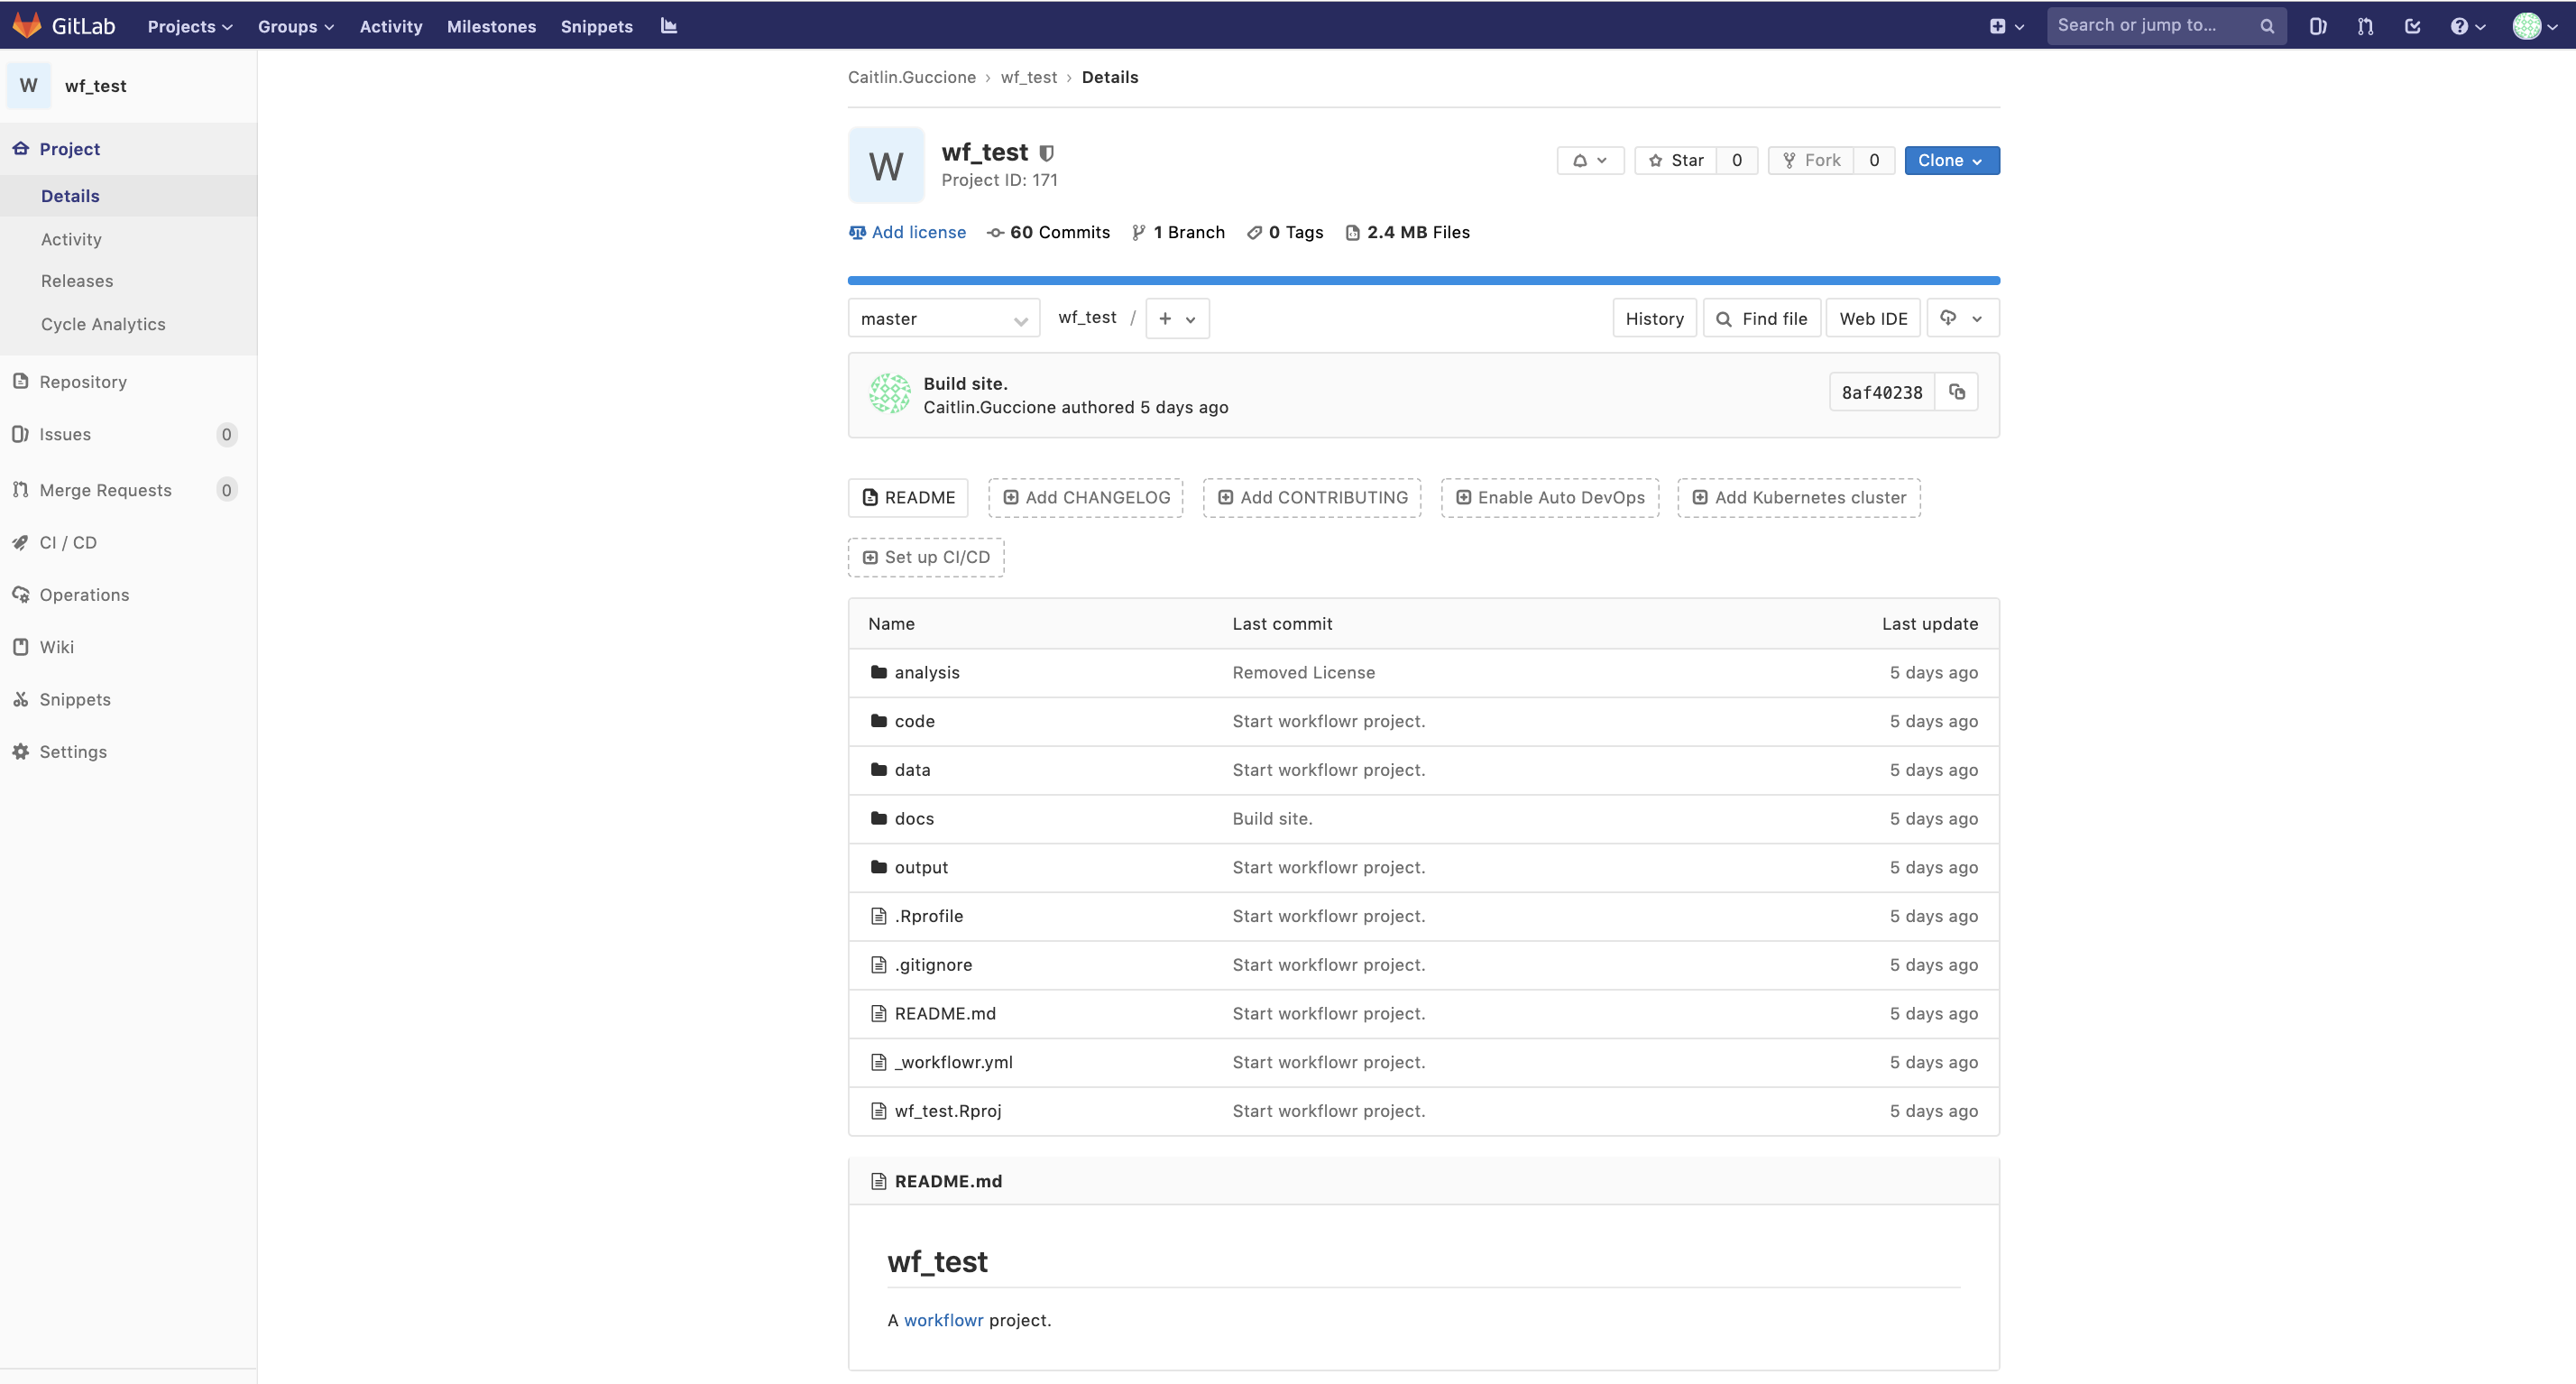
\includegraphics[width=1\linewidth]{images/Workflow_Photos/screen_shot} 

}

\caption{Example of a Workflowr connection on GitLab}\label{fig:a3}
\end{figure}

\hypertarget{adding-new-files}{%
\subsubsection{Adding New Files}\label{adding-new-files}}

\hypertarget{creating-new-files}{%
\paragraph{Creating New Files}\label{creating-new-files}}

Make sure you are inside the PROJECT\_NAME project inside RStudio

In \texttt{Console} tab type:

\begin{Shaded}
\begin{Highlighting}[]
\KeywordTok{wflow_open}\NormalTok{(}\StringTok{"analysis/NEW_FILE.Rmd"}\NormalTok{)}
\end{Highlighting}
\end{Shaded}

\begin{itemize}
\tightlist
\item
  This command creates a new Rmd file and then opens it for your convenience.
\end{itemize}

If we now want to see the HTML version of our file then we have two options:

\begin{enumerate}
\def\labelenumi{\arabic{enumi}.}
\tightlist
\item
  In \texttt{Console} tab type:
\end{enumerate}

\begin{Shaded}
\begin{Highlighting}[]
\KeywordTok{wflow_build}\NormalTok{()}
\end{Highlighting}
\end{Shaded}

\begin{itemize}
\tightlist
\item
  You can add specific files to this command or simply leave it empty
\item
  This produces a small view of your website right on RStudio
\end{itemize}

\begin{enumerate}
\def\labelenumi{\arabic{enumi}.}
\setcounter{enumi}{1}
\tightlist
\item
  Press the `Knit' button in RStudio as shown below:
\end{enumerate}

\begin{figure}

{\centering 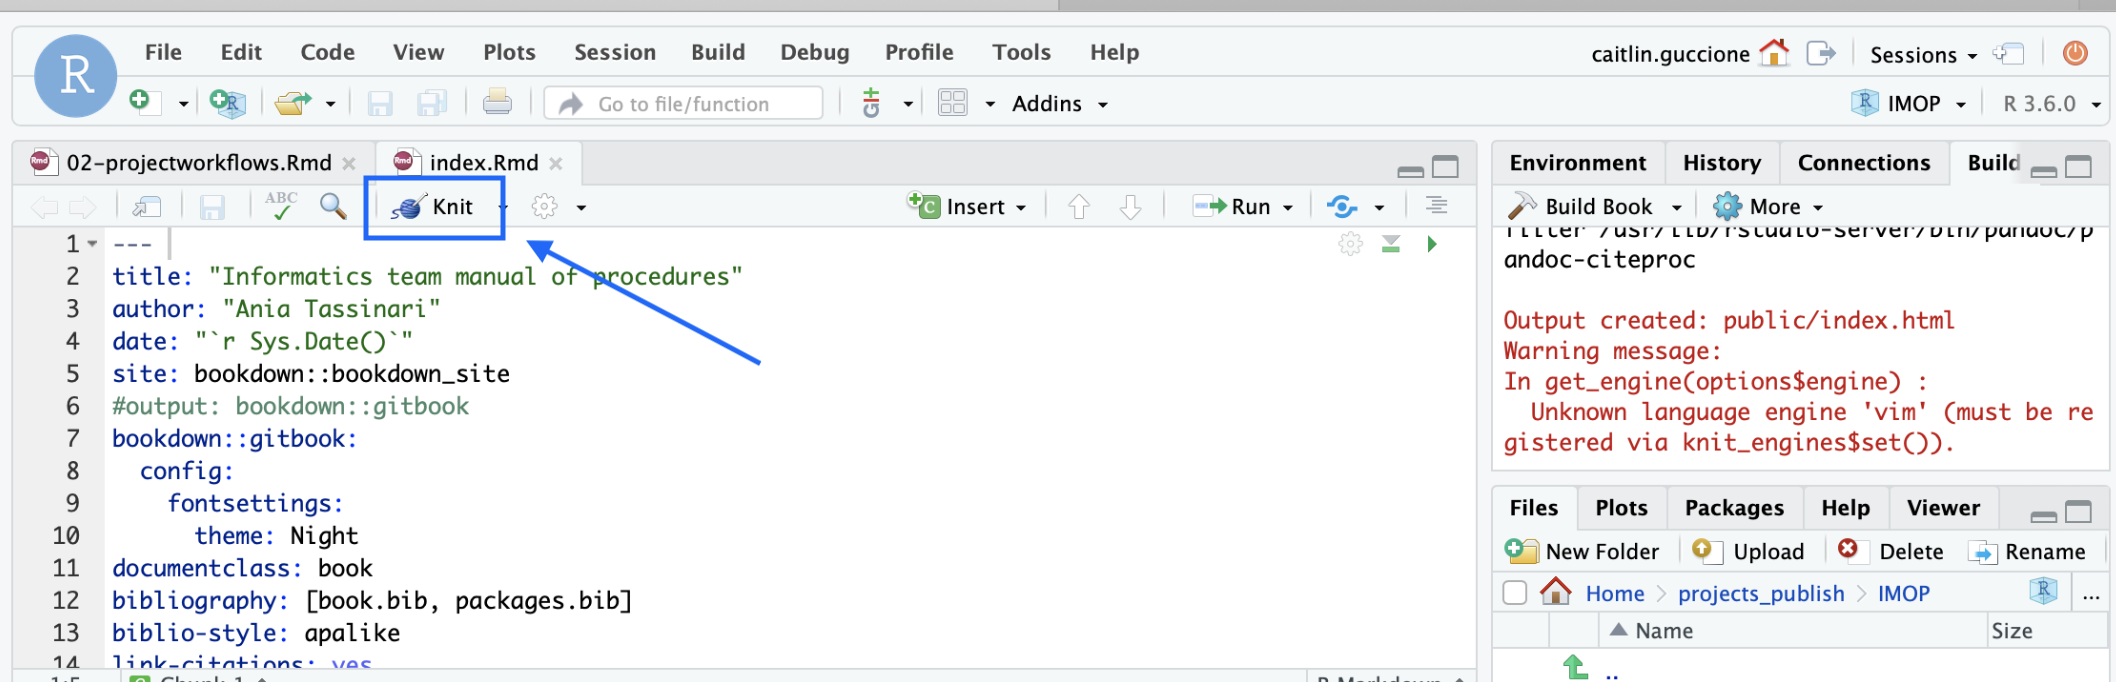
\includegraphics[width=0.8\linewidth]{images/Workflow_Photos/knit_arrow} 

}

\caption{ Display of where the Knit button is located in RStudio}\label{fig:d2}
\end{figure}

\begin{itemize}
\tightlist
\item
  This produces a large web version of your current HTML file
\end{itemize}

These steps will simply change the local HTML file, but in order to make this public and add it to GitLab, we need to update our changes.

\hypertarget{update-your-changes}{%
\paragraph{Update your Changes}\label{update-your-changes}}

\begin{enumerate}
\def\labelenumi{\arabic{enumi}.}
\tightlist
\item
  Check the status to see what needs to be updated, in the \texttt{Console} tab, type:
\end{enumerate}

\begin{Shaded}
\begin{Highlighting}[]
\KeywordTok{wflow_status}\NormalTok{()}
\end{Highlighting}
\end{Shaded}

This can also be done by looking at the red checks on the workflowr section of your live page as shown below:

\begin{figure}

{\centering 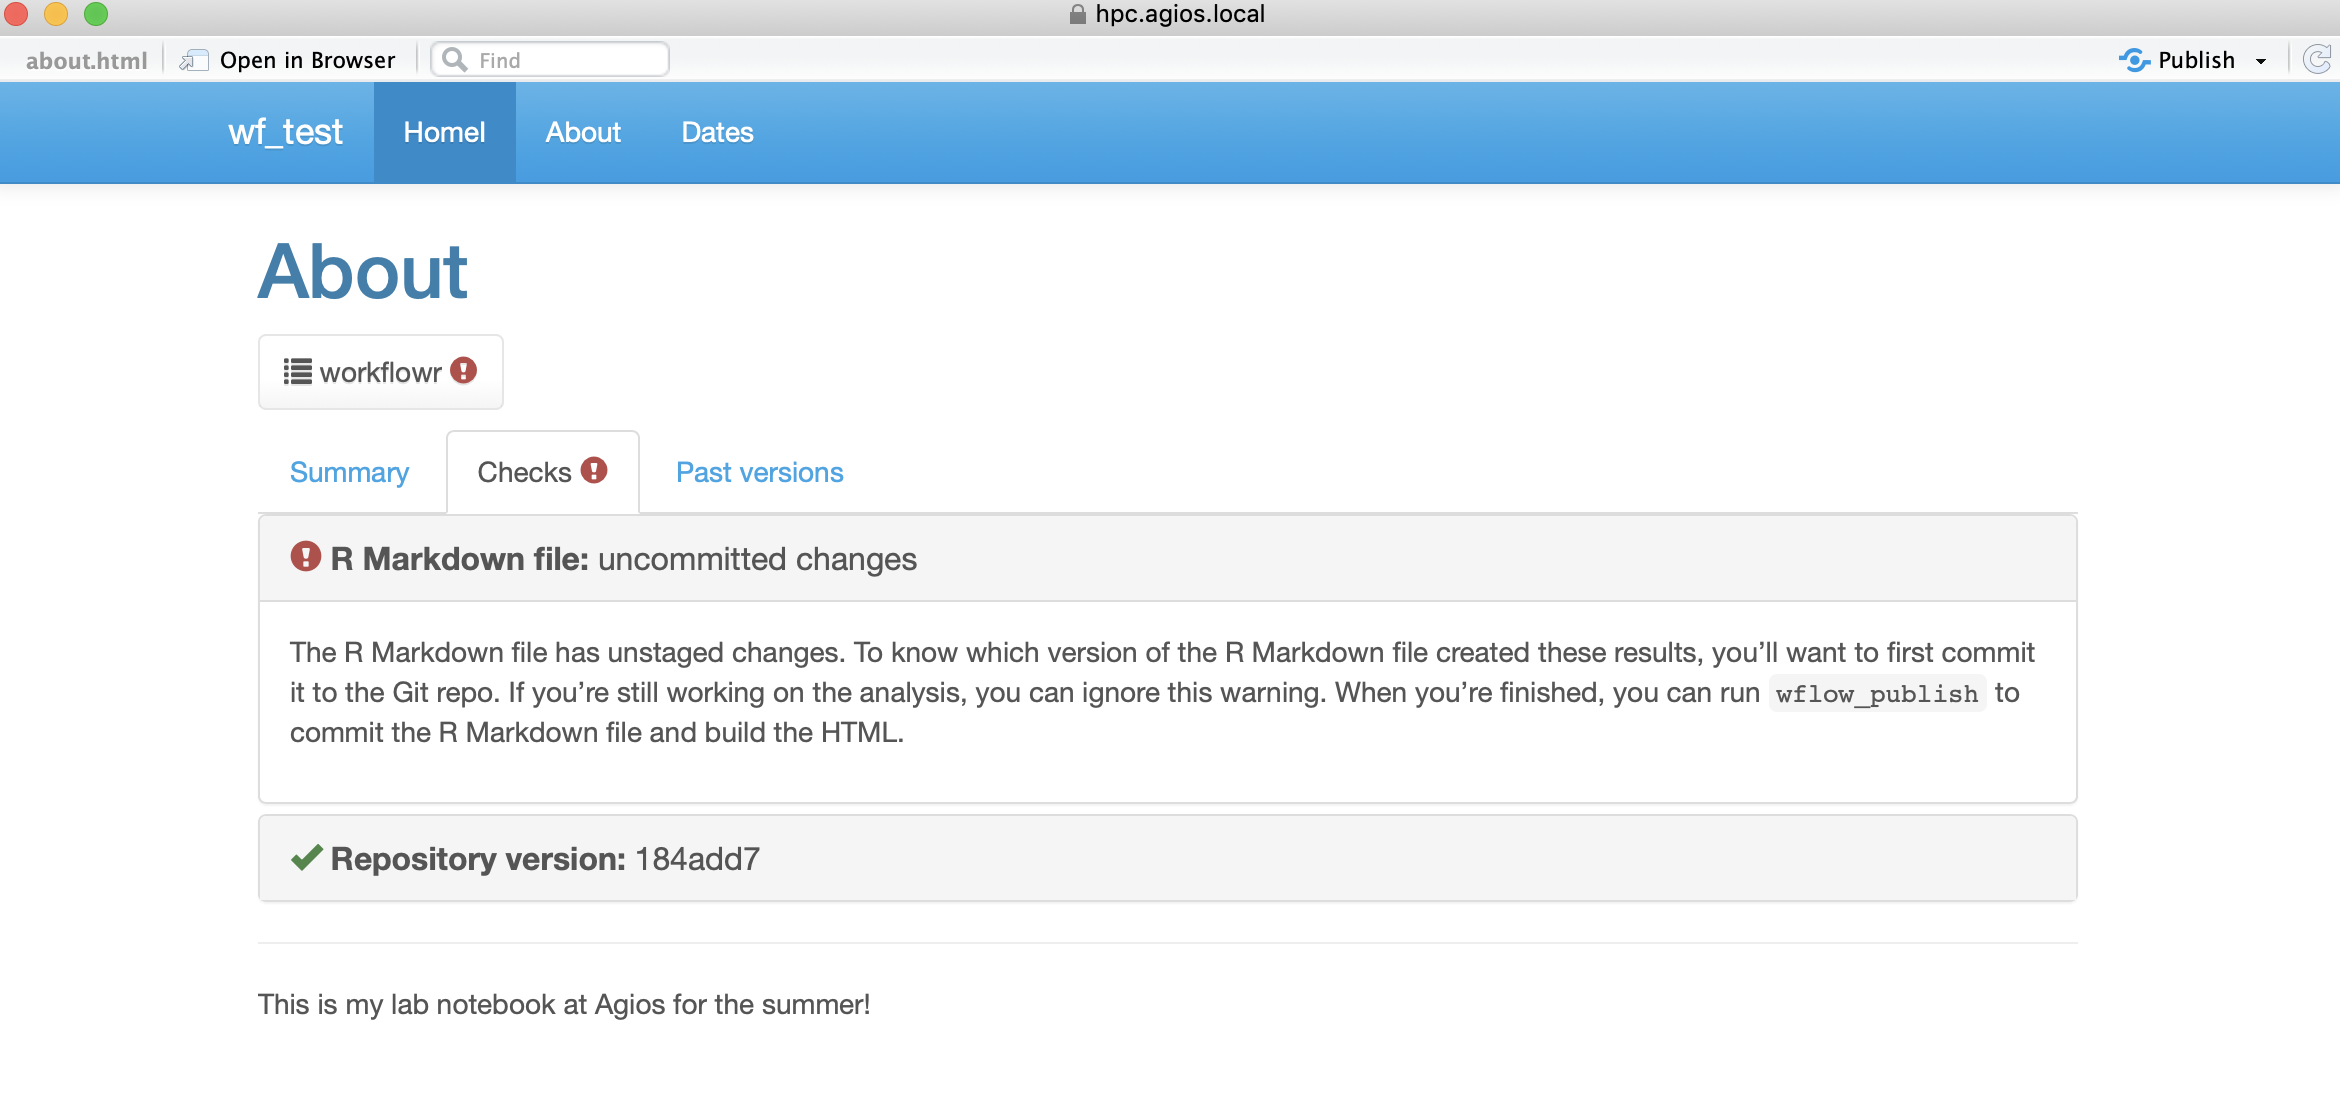
\includegraphics[width=0.9\linewidth]{images/Workflow_Photos/red_checks} 

}

\caption{A demenstration of a live Workflowr page}\label{fig:d4}
\end{figure}

\begin{enumerate}
\def\labelenumi{\arabic{enumi}.}
\setcounter{enumi}{1}
\tightlist
\item
  Make the appropriate HTML files public and updated, in the \texttt{Console} tab, type:
\end{enumerate}

\begin{Shaded}
\begin{Highlighting}[]
\KeywordTok{wflow_publish}\NormalTok{(}\KeywordTok{c}\NormalTok{(}\StringTok{"analysis/index.Rmd"}\NormalTok{, }
    \StringTok{"analysis/NEW_FILE.Rmd"}\NormalTok{), }\StringTok{"Add my first file"}\NormalTok{)}
\end{Highlighting}
\end{Shaded}

\begin{itemize}
\tightlist
\item
  This is the same format found on the \protect\hyperlink{publish-website}{\textbf{Publish Website}} tab of this page and so you can customize it in the same way
\end{itemize}

There is one exception to this and it's when you want to make updates to the \texttt{\_site.yml} file found in the \texttt{analysis} folder. This file controls the style on the top of every page of your website. In this case, you want to update all HTML files even though their Rmd files aren't changed.

In that case, use this,

\begin{Shaded}
\begin{Highlighting}[]
\KeywordTok{wflow_publish}\NormalTok{(}\StringTok{"analysis/_site.yml"}\NormalTok{, }
    \StringTok{"Change the theme"}\NormalTok{, }\DataTypeTok{republish =} \OtherTok{TRUE}\NormalTok{)}
\end{Highlighting}
\end{Shaded}

\begin{enumerate}
\def\labelenumi{\arabic{enumi}.}
\setcounter{enumi}{2}
\tightlist
\item
  Push the final changes to GitLab
\end{enumerate}

As we did previously in the \texttt{Publish\ Website}, in the \texttt{Terminal} tab, type:

\begin{Shaded}
\begin{Highlighting}[]
\NormalTok{git push}
\end{Highlighting}
\end{Shaded}

\hypertarget{adding-workflowr-to-new-file}{%
\paragraph{Adding Workflowr to New File}\label{adding-workflowr-to-new-file}}

If you want the workflowr setup which is found on all the other pages, then replace the --- part of the file with the following code:

\begin{Shaded}
\begin{Highlighting}[]
            \OperatorTok{---}
\StringTok{            }\NormalTok{title}\OperatorTok{:}\StringTok{ "Home"}
\NormalTok{            site}\OperatorTok{:}\StringTok{ }\NormalTok{workflowr}\OperatorTok{::}\NormalTok{wflow_site}
\NormalTok{            output}\OperatorTok{:}
\StringTok{              }\NormalTok{workflowr}\OperatorTok{::}\NormalTok{wflow_html}\OperatorTok{:}
\StringTok{                }\NormalTok{toc}\OperatorTok{:}\StringTok{ }\NormalTok{false}
\NormalTok{            editor_options}\OperatorTok{:}
\StringTok{              }\NormalTok{chunk_output_type}\OperatorTok{:}\StringTok{ }\NormalTok{console}
            \OperatorTok{---}
\end{Highlighting}
\end{Shaded}

\begin{center}\includegraphics[width=0.6\linewidth]{images/Workflow_Photos/uMadeIt2} \end{center}

\hypertarget{quick-additions-to-improve-your-workflowr}{%
\subsubsection{Quick Additions to Improve your Workflowr}\label{quick-additions-to-improve-your-workflowr}}

\hypertarget{adding-packrat-1}{%
\paragraph{Adding PackRat}\label{adding-packrat-1}}

PackRat records or saves the exact package versions that you depend on and stores them in GitLab.

\begin{enumerate}
\def\labelenumi{\arabic{enumi}.}
\tightlist
\item
  Install PackRat
\end{enumerate}

\begin{Shaded}
\begin{Highlighting}[]
\KeywordTok{install.packages}\NormalTok{(}\StringTok{"packrat"}\NormalTok{)}
\end{Highlighting}
\end{Shaded}

\begin{enumerate}
\def\labelenumi{\arabic{enumi}.}
\setcounter{enumi}{1}
\item
  Add PackRat to Existing Project

  \begin{itemize}
  \tightlist
  \item
    Go to \texttt{Tools}
  \item
    Click on \texttt{Project\ Options}
  \item
    Click \texttt{Add\ PackRat} then check \texttt{Use\ PackRat\ for\ this\ project}
  \item
    Now, check the following boxes (shown in the image below) and tap \texttt{OK} *:
  \end{itemize}
\end{enumerate}

\begin{itemize}
\tightlist
\item
  This step may take a while if you have a number of packages you are backing up.
\end{itemize}

\begin{center}\includegraphics[width=0.6\linewidth]{images/Workflow_Photos/packRat} \end{center}

\begin{itemize}
\tightlist
\item
  This step may take a while if you have a large amount of packages you want to back up
\end{itemize}

\begin{enumerate}
\def\labelenumi{\arabic{enumi}.}
\setcounter{enumi}{2}
\tightlist
\item
  A panel called PackRat will now appear under packages

  \begin{itemize}
  \tightlist
  \item
    It will automatically notify you if packrat has a package that you don't and then prompt you to download it
  \end{itemize}
\item
  It also gives you the option to clean un-used packages so that packrat doesn't get too cluttered
\end{enumerate}

\hypertarget{update-session-information-function-1}{%
\paragraph{Update Session Information Function}\label{update-session-information-function-1}}

The following steps simply add more information to your \texttt{Session\ Info} button found at the bottom of your workflowr. For more information about how to further customize the \texttt{Session\ Info} output click \href{https://jdblischak.github.io/workflowr/articles/wflow-02-customization.html}{here}

Add the following line to your \texttt{\_workflowr.yml} file :

\begin{Shaded}
\begin{Highlighting}[]
\NormalTok{sessioninfo}\OperatorTok{:}\StringTok{"devtools::session_info()"}
\end{Highlighting}
\end{Shaded}

\hypertarget{publish-to-gitlab-without-rebuilding-sites-1}{%
\paragraph{Publish to GitLab without Rebuilding Sites}\label{publish-to-gitlab-without-rebuilding-sites-1}}

A quicker way to push to GitLab without rebuilding your website.

\begin{enumerate}
\def\labelenumi{\arabic{enumi}.}
\tightlist
\item
  Edit the Rmd file and save your changes
\item
  Run one of the following commands (doesn't matter which one you select)

  \begin{itemize}
  \tightlist
  \item
    \texttt{wflow\_build()}

    \begin{itemize}
    \tightlist
    \item
      It doesn't matter if we build other files, they won't be added to git unless we add them in the next step
    \end{itemize}
  \item
    \texttt{wflow\_build("file.rmd")}
  \item
    Knit the file
  \end{itemize}
\item
  \texttt{wflow\_git\_commit("file.rmd",\ "This\ is\ your\ commit\ message")}
\item
  Flip into the terminal and run \texttt{git\ push()}
\end{enumerate}

\hypertarget{create-a-live-shareable-webpage}{%
\subsubsection{Create a LIVE Shareable Webpage}\label{create-a-live-shareable-webpage}}

Below are a few ways to share your project with others.

\hypertarget{a-simple-trick}{%
\paragraph{A Simple Trick}\label{a-simple-trick}}

This is the simplest way to share your workflowr page at the moment. In the future, we are hoping to have a cleaner way to do so.

\begin{enumerate}
\def\labelenumi{\arabic{enumi}.}
\tightlist
\item
  Have the new user clone your page on GitLab
\item
  Open the \texttt{docs} folder
\item
  Click on the \texttt{index.html} file
\end{enumerate}

\hypertarget{gitlab-pages}{%
\paragraph{GitLab Pages}\label{gitlab-pages}}

\href{https://about.gitlab.com/product/pages/}{GitLab Pages} isn't currently available on Agio's GitLab. As soon as it is, we will add updates on how to simply set-up and share GitLab pages. If you would like to experiment with GitHub pages you may do so on your personal GitHub account, once GitLab pages are up and running they should behave in almost the same way.

\hypertarget{beaker-browser}{%
\paragraph{Beaker Browser}\label{beaker-browser}}

\href{https://beakerbrowser.com/}{Beaker Browser} is a simple way to deploy a webpage from your computer without a server. We attempted to use Beaker Browser though we found it had a few setbacks and that other methods may be simpler. If you want to try it out for yourself, the link above is very straightforward.

The comparison above between GitLab pages and Beaker Browser:

\begin{longtable}[]{@{}ll@{}}
\toprule
\begin{minipage}[b]{0.47\columnwidth}\raggedright
GitLab Pages\strut
\end{minipage} & \begin{minipage}[b]{0.47\columnwidth}\raggedright
Beaker Browser\strut
\end{minipage}\tabularnewline
\midrule
\endhead
\begin{minipage}[t]{0.47\columnwidth}\raggedright
Slightly complex setup\strut
\end{minipage} & \begin{minipage}[t]{0.47\columnwidth}\raggedright
Simpler setup\strut
\end{minipage}\tabularnewline
\begin{minipage}[t]{0.47\columnwidth}\raggedright
Automatically updates changes, since it's already linked to Git\strut
\end{minipage} & \begin{minipage}[t]{0.47\columnwidth}\raggedright
Not a clear path to Git and thus must manually update changes\strut
\end{minipage}\tabularnewline
\begin{minipage}[t]{0.47\columnwidth}\raggedright
Well documented\strut
\end{minipage} & \begin{minipage}[t]{0.47\columnwidth}\raggedright
Little documentation\strut
\end{minipage}\tabularnewline
\begin{minipage}[t]{0.47\columnwidth}\raggedright
Easy to share internally through GitLab\strut
\end{minipage} & \begin{minipage}[t]{0.47\columnwidth}\raggedright
Have to download Beaker in order to view the webpage\strut
\end{minipage}\tabularnewline
\bottomrule
\end{longtable}

\hypertarget{styling-the-webpage}{%
\subsubsection{Styling the Webpage}\label{styling-the-webpage}}

\hypertarget{helpful-links}{%
\paragraph{Helpful Links}\label{helpful-links}}

If you already have an idea of what you would like to change, below are a few very helpful resources filled with information:

\begin{itemize}
\tightlist
\item
  This resource is a great place to start because it has all basics of Rmd syntax and I used it as a cheat sheet along the way.

  \begin{itemize}
  \tightlist
  \item
    \href{https://rmarkdown.rstudio.com/authoring_basics.html}{Rmd Cheat Sheet}
  \end{itemize}
\item
  This is an entire book all about Rmd and how to use it. I found it rather lengthy but very helpful.

  \begin{itemize}
  \tightlist
  \item
    \href{https://bookdown.org/yihui/rmarkdown/html-document.html\#appearance_and_style}{Rmd Thorough Guide}
  \end{itemize}
\item
  If something isn't quite working right you may have run into a workflowr issue in which cause their FAQ's page is helpful.

  \begin{itemize}
  \tightlist
  \item
    \href{https://jdblischak.github.io/workflowr/articles/wflow-05-faq.html}{Workflowr FAQ's}
  \end{itemize}
\end{itemize}

\hypertarget{changing-the-theme}{%
\paragraph{Changing the Theme}\label{changing-the-theme}}

Changing the theme modifies the overall appearance of the webpage and is a quick and easy way to spice up the page.

\begin{enumerate}
\def\labelenumi{\arabic{enumi}.}
\tightlist
\item
  Go into your \texttt{analysis/\_site.yml} file
\item
  Underneath \texttt{ouput} add \texttt{theme\ =\ cerulean} as shown below:

  \begin{itemize}
  \tightlist
  \item
    The cerulean theme matches Agios colors
  \end{itemize}
\end{enumerate}

\begin{Shaded}
\begin{Highlighting}[]
\NormalTok{output}\OperatorTok{:}\NormalTok{theme}\OperatorTok{:}\NormalTok{cerulean}
\end{Highlighting}
\end{Shaded}

\begin{enumerate}
\def\labelenumi{\arabic{enumi}.}
\setcounter{enumi}{2}
\tightlist
\item
  Choose your theme

  \begin{itemize}
  \tightlist
  \item
    The following themes are available : ``default'', ``cerulean'', ``journal'', ``flatly'', ``darkly'', ``readable'', ``spacelab'', ``united'', ``cosmo'', ``lumen'', ``paper'', ``sandstone'', ``simplex'', ``yeti''
  \item
    You can view how they look here: \href{https://bootswatch.com/}{Themes}
  \end{itemize}
\item
  Preview your theme using,
\end{enumerate}

\begin{Shaded}
\begin{Highlighting}[]
\KeywordTok{wflow_build}\NormalTok{()}
\end{Highlighting}
\end{Shaded}

\begin{enumerate}
\def\labelenumi{\arabic{enumi}.}
\setcounter{enumi}{4}
\tightlist
\item
  Update your website by running,

  \begin{itemize}
  \tightlist
  \item
    This will rebuild every HTML file even if their corresponding Rmd file hasn't been updated
  \end{itemize}
\end{enumerate}

\begin{Shaded}
\begin{Highlighting}[]
\KeywordTok{wflow_publish}\NormalTok{(}\StringTok{"analysis/_site.yml"}\NormalTok{, }
    \StringTok{"Change the theme"}\NormalTok{, }\DataTypeTok{republish =} \OtherTok{TRUE}\NormalTok{)}
\end{Highlighting}
\end{Shaded}

The following website will also walk you through changing the theme: \href{https://jdblischak.github.io/workflowr/articles/wflow-02-customization.html\#changing-the-theme}{Themes Overview}

\hypertarget{adding-photos}{%
\paragraph{Adding Photos}\label{adding-photos}}

Although this may seem like a simple task, it is a bit challenging since we are using Workflowr

\begin{enumerate}
\def\labelenumi{\arabic{enumi}.}
\tightlist
\item
  Create a \texttt{photos} folder inside the \texttt{docs} folder and add your photo there:
\end{enumerate}

\begin{Shaded}
\begin{Highlighting}[]
\KeywordTok{dir.create}\NormalTok{(}\StringTok{"docs/photos"}\NormalTok{)}
\end{Highlighting}
\end{Shaded}

\begin{enumerate}
\def\labelenumi{\arabic{enumi}.}
\setcounter{enumi}{1}
\tightlist
\item
  Include the following command wherever you want your graphic to appear:
\end{enumerate}

\begin{flushleft}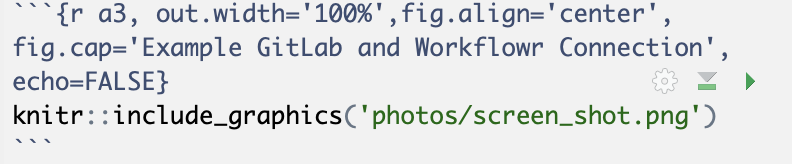
\includegraphics[width=0.5\linewidth]{images/Workflow_Photos/photoExample} \end{flushleft}

\begin{verbatim}
+ Adjusting `out.width` changes the size of the photo
\end{verbatim}

\begin{enumerate}
\def\labelenumi{\arabic{enumi}.}
\setcounter{enumi}{2}
\tightlist
\item
  View the images on the webpage
\end{enumerate}

\begin{Shaded}
\begin{Highlighting}[]
\KeywordTok{wflow_build}\NormalTok{()}
\end{Highlighting}
\end{Shaded}

\begin{enumerate}
\def\labelenumi{\arabic{enumi}.}
\setcounter{enumi}{3}
\tightlist
\item
  Add to GitLab

  \begin{itemize}
  \tightlist
  \item
    We need to push the actual photo to GitLab using \texttt{wflow\_git\_commit} and then we can use \texttt{wflow\_publish} to automatically push the rest of the files to GitLab
  \end{itemize}
\end{enumerate}

\begin{Shaded}
\begin{Highlighting}[]
\KeywordTok{wflow_git_commit}\NormalTok{(}\StringTok{"docs/assets/external.png"}\NormalTok{, }
    \StringTok{"Add external image of ..."}\NormalTok{)}
\KeywordTok{wflow_publish}\NormalTok{()}
\end{Highlighting}
\end{Shaded}

\hypertarget{blogdown}{%
\paragraph{Blogdown}\label{blogdown}}

\href{https://bookdown.org/yihui/blogdown/a-quick-example.html}{Blogdown} is another way that you can customize your workflowr page more easily. It is a combination of the well known blogdown and workflowr.

You can clone the following repo on GitHub if you want to try it out: \href{https://github.com/docmanny/workflowr-blogdown-experiment}{Blogdown/Workflowr Repo}

\begin{center}\rule{0.5\linewidth}{\linethickness}\end{center}

\hypertarget{set-up-workflow-and-executing}{%
\subsection{Set Up Workflow and Executing}\label{set-up-workflow-and-executing}}

\hypertarget{create-a-folder-for-your-newproject}{%
\subsubsection{\texorpdfstring{Create a folder for your \emph{newproject}}{Create a folder for your newproject}}\label{create-a-folder-for-your-newproject}}

Come up with a project structure you like and stick with it.

\hypertarget{copy-from-a-previously-created-template-folder}{%
\paragraph{Copy from a previously created template folder}\label{copy-from-a-previously-created-template-folder}}

Use \texttt{cp\ -r\ project\_template\ newproject}, where \texttt{project\_template} has structure:

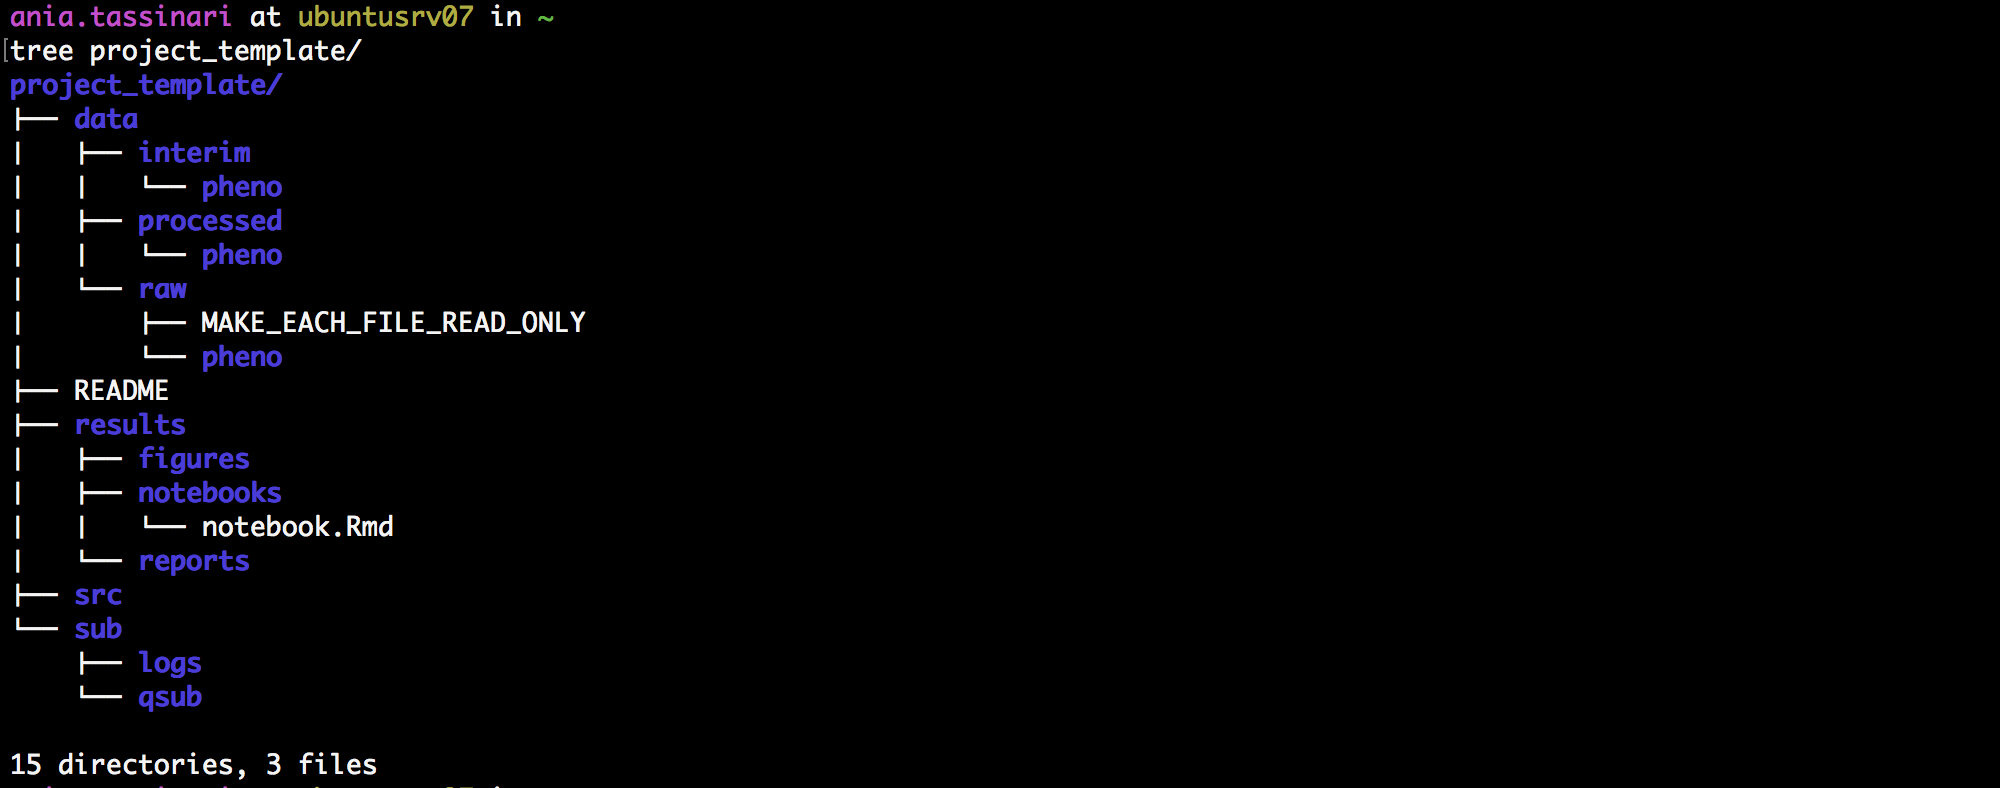
\includegraphics[width=0.8\linewidth]{images/projectstructure}

\hypertarget{use-a-bash-script}{%
\paragraph{\texorpdfstring{Use a \texttt{bash} script}{Use a bash script}}\label{use-a-bash-script}}

Call \texttt{./setup\_project.sh\ newproject}, where \texttt{setup\_project.sh} is:

Don't forget!
- Fill project README
- Adapt structure to project needs
- Exclude data and other large files from git using \texttt{.gitignore} (see next section)
- Make files in \texttt{data/raw} read-only with \texttt{chmod\ -w}

Project organization ideas:
\url{http://projecttemplate.net/getting_started.html}
Packaging data analytical work reproducibly using R (and friends)
R workflow fun
Cookiecutter Data Science

\hypertarget{set-up-a-repository-for-your-code-on-agios-secure-gitlab}{%
\subsubsection{Set up a repository for your code on Agios' secure GitLab}\label{set-up-a-repository-for-your-code-on-agios-secure-gitlab}}

Create a new project at http://ceres.agios.com (Mark P. can help)

\hypertarget{set-up-a-repository-for-your-code-locally-and-link-to-gitlab}{%
\subsubsection{Set up a repository for your code locally and link to GitLab}\label{set-up-a-repository-for-your-code-locally-and-link-to-gitlab}}

In your \emph{newproject} folder on command line execute (modify user name):

\begin{Shaded}
\begin{Highlighting}[]
\NormalTok{git add .}
\NormalTok{git commit }\OperatorTok{-}\NormalTok{am }\StringTok{'initial commit'}
\NormalTok{git remote add origin git}\OperatorTok{@}\NormalTok{ceres.agios.com}\OperatorTok{:}\NormalTok{User.Name}\OperatorTok{/}\NormalTok{newproject.git}
\NormalTok{git push }\OperatorTok{-}\NormalTok{u origin master }
\end{Highlighting}
\end{Shaded}

\hypertarget{set-up-an-r-project-in-rstudio}{%
\subsubsection{Set up an R project in RStudio}\label{set-up-an-r-project-in-rstudio}}

Choose Existing Directory (\emph{newproject})

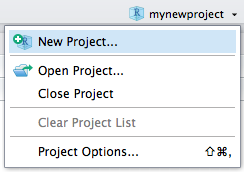
\includegraphics[width=0.6\linewidth]{images/newproject0}
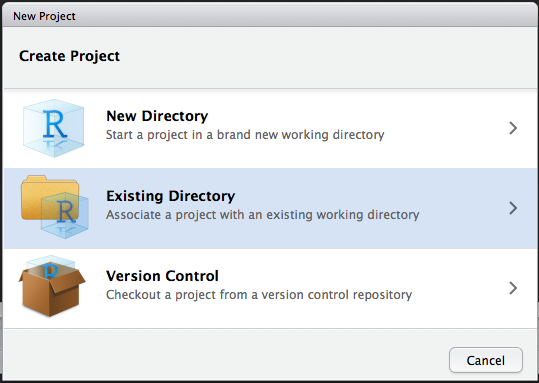
\includegraphics[width=0.6\linewidth]{images/newproject}

\hypertarget{analysis-in-r-and-rstudio}{%
\subsubsection{Analysis in R and RStudio}\label{analysis-in-r-and-rstudio}}

\textbf{Data:}

\begin{itemize}
\tightlist
\item
  Raw data:

  \begin{itemize}
  \tightlist
  \item
    If accessed from the web, include url, description, and date accessed in README
  \end{itemize}
\item
  Processed:

  \begin{itemize}
  \tightlist
  \item
    Processed data should be named so it is easy to see which script generated the data

    \begin{itemize}
    \tightlist
    \item
      Can add file descriptions to \texttt{filename.README} and place processing script in the same directory as data (works well for preprocessing steps, like alignments, etc)
    \end{itemize}
  \item
    Processed data should be tidy
  \end{itemize}
\end{itemize}

\textbf{Code:}

\begin{itemize}
\tightlist
\item
  Place (almost) all intermediate scripts in \texttt{newproject/src/}
\item
  Any chunks of code frequently reused in the analysis should be converted into functions, saved in \texttt{newproject/src/functions.R}, and sourced in scripts, notebooks and reports.\\
\item
  Use Google's R Style Guide or The tidyverse styleguide to format your code and make it easier to read (if need be run code through formatR)
\end{itemize}

\textbf{Figures:}

\begin{itemize}
\tightlist
\item
  Exploratory:

  \begin{itemize}
  \tightlist
  \item
    Don't have to be pretty
  \item
    Can be embedded in report/notebook
  \end{itemize}
\item
  Final:

  \begin{itemize}
  \tightlist
  \item
    Should be polished and saved in \texttt{newproject/results/figures/}
  \end{itemize}
\end{itemize}

\textbf{Scripts:}

\begin{itemize}
\tightlist
\item
  Raw:

  \begin{itemize}
  \tightlist
  \item
    May be less commented (but comments help you!)
  \item
    May be multiple versions
  \item
    May include analyses that are later discarded
  \end{itemize}
\item
  Final:

  \begin{itemize}
  \tightlist
  \item
    Clearly commented
  \item
    Small comments liberally - what, when, why, how
  \item
    Bigger commented blocks for whole sections
  \item
    Include processing details
  \item
    Only analyses that appear in the final write-up
  \end{itemize}
\end{itemize}

\textbf{Notebooks and reports:}

\begin{itemize}
\item
  R markdown files can be used to generate reproducible reports
\item
  Text and R code are integrated
\item
  Notebooks:

  \begin{itemize}
  \tightlist
  \item
    intermediate
  \item
    may use one per day or one per subanalysis
  \item
    documents all atempts
  \end{itemize}
\item
  Reports:

  \begin{itemize}
  \tightlist
  \item
    final methods and results only
  \item
    good for sharing
  \end{itemize}
\end{itemize}

Adapted from: Reproducible Research at Coursera

\hypertarget{version-control-in-git-and-gitlab}{%
\subsubsection{Version control in git and GitLab}\label{version-control-in-git-and-gitlab}}

Adopt a branching workflow appropriate for the project and team size, and stick to it.

\url{gitforsmallteams}

Reprinted from: Git workflow for small teams. Link currently is password protected.

\textbf{\texttt{git} and \texttt{git-workflow} resources:}
Learn git
Git branching model
GitFlow

\hypertarget{keeping-track-of-enviroment}{%
\subsubsection{Keeping track of enviroment}\label{keeping-track-of-enviroment}}

Use \texttt{devtools::session\_info()}

or \texttt{sessionInfo()}

or \texttt{docker} with \texttt{rrtools}

\hypertarget{toolbox}{%
\section{Toolbox}\label{toolbox}}

\hypertarget{command-line-tools}{%
\subsection{Command Line Tools}\label{command-line-tools}}

\hypertarget{bioinformatics}{%
\subsubsection{Bioinformatics}\label{bioinformatics}}

\hypertarget{get-average-read-length-from-a-.bam-file}{%
\paragraph{\texorpdfstring{Get average read length from a \texttt{.bam} file}{Get average read length from a .bam file}}\label{get-average-read-length-from-a-.bam-file}}

\begin{Shaded}
\begin{Highlighting}[]
\ExtensionTok{samtools}\NormalTok{ view sorted.bam }\KeywordTok{|} \FunctionTok{head}\NormalTok{ -n 1000000 }\KeywordTok{|} \FunctionTok{cut}\NormalTok{ -f 10 }\KeywordTok{|} \FunctionTok{perl}\NormalTok{ -ne }\StringTok{'chomp;print length($_) . "\textbackslash{}n"'} \KeywordTok{|} \FunctionTok{sort} \KeywordTok{|} \FunctionTok{uniq}\NormalTok{ -c}
\end{Highlighting}
\end{Shaded}

\hypertarget{docker}{%
\subsubsection{Docker}\label{docker}}

\hypertarget{basic-commands}{%
\paragraph{Basic commands}\label{basic-commands}}

Here are a few helpful commands for working with \texttt{docker} images
docker ps -a \# Lists containers (and tells you which images they are spun from)
docker images \# Lists images\\
docker rm \# Removes a container

docker rmi \# Removes an image
\# Will fail if there is a running instance of that image i.e.~container

docker rmi -f \# Forces removal of image even if it is referenced in multiple repositories,
\# i.e.~same image id given multiple names/tags
\# Will still fail if there is a docker container referencing image

\hypertarget{pruning}{%
\paragraph{Pruning}\label{pruning}}

\begin{Shaded}
\begin{Highlighting}[]
\CommentTok{# remove dangling images }
\NormalTok{docker rmi }\OperatorTok{$}\NormalTok{(docker images }\OperatorTok{--}\NormalTok{filter “}\DataTypeTok{dangling=}\NormalTok{true” }\OperatorTok{-}\NormalTok{q }\OperatorTok{--}\NormalTok{no}\OperatorTok{-}\NormalTok{trunc)}

\CommentTok{# find other untagged images (with possible children) (<none>:<none>)}
\NormalTok{docker images }\OperatorTok{-}\NormalTok{a }\OperatorTok{|}\StringTok{ }\NormalTok{grep }\StringTok{"none"} \OperatorTok{|}\StringTok{ }\NormalTok{awk }\StringTok{'\{print $3\}'}

\CommentTok{# try removing them}
\NormalTok{docker rmi }\OperatorTok{$}\NormalTok{(docker images }\OperatorTok{-}\NormalTok{a }\OperatorTok{|}\StringTok{ }\NormalTok{grep }\StringTok{"none"} \OperatorTok{|}\StringTok{ }\NormalTok{awk }\StringTok{'\{print $3\}'}\NormalTok{)}

\CommentTok{# if any left because of clingy children, get __parent.ID__ (ID of untagged image) and then:}
\CommentTok{# example: docker inspect --format='\{\{.Id\}\} \{\{.Parent\}\}' $(docker images --filter since=14a1e7116365 -q)}
\NormalTok{docker inspect }\OperatorTok{--}\NormalTok{format=}\StringTok{'\{\{.Id\}\} \{\{.Parent\}\}'} \OperatorTok{$}\NormalTok{(docker images }\OperatorTok{--}\NormalTok{filter }\DataTypeTok{since=}\NormalTok{__parent.id__ }\OperatorTok{-}\NormalTok{q)}

\CommentTok{# then remove listed __children.id__ one by one}
\CommentTok{# example: docker rmi 382096f13260254f3c472bf63f063b8ecbc2d4cc06fe7a940d6fbd4636ef77b1}
\NormalTok{docker rmi __child.id__}
\end{Highlighting}
\end{Shaded}

\hypertarget{file-system}{%
\subsubsection{File system}\label{file-system}}

\hypertarget{list-top-5-largest-files}{%
\paragraph{List top 5 largest files}\label{list-top-5-largest-files}}

\begin{Shaded}
\begin{Highlighting}[]
\NormalTok{du }\OperatorTok{-}\NormalTok{a }\OperatorTok{/}\NormalTok{path}\OperatorTok{/}\NormalTok{to}\OperatorTok{/}\NormalTok{my}\OperatorTok{/}\NormalTok{dir}\OperatorTok{/}\StringTok{ }\ErrorTok{|}\StringTok{ }\NormalTok{sort }\OperatorTok{-}\NormalTok{n }\OperatorTok{-}\NormalTok{r }\OperatorTok{|}\StringTok{ }\NormalTok{head }\OperatorTok{-}\NormalTok{n }\DecValTok{5}
\end{Highlighting}
\end{Shaded}

Example:

\begin{Shaded}
\begin{Highlighting}[]
\NormalTok{du }\OperatorTok{-}\NormalTok{a }\OperatorTok{/}\NormalTok{bin }\OperatorTok{|}\StringTok{ }\NormalTok{sort }\OperatorTok{-}\NormalTok{n }\OperatorTok{-}\NormalTok{r }\OperatorTok{|}\StringTok{ }\NormalTok{head }\OperatorTok{-}\NormalTok{n }\DecValTok{5}
\end{Highlighting}
\end{Shaded}

\hypertarget{list-files-in-a-folder-separated-by-delimeter}{%
\paragraph{List files in a folder separated by delimeter}\label{list-files-in-a-folder-separated-by-delimeter}}

\begin{Shaded}
\begin{Highlighting}[]
\NormalTok{ls }\DecValTok{-1} \OperatorTok{/}\NormalTok{path}\OperatorTok{/}\NormalTok{to}\OperatorTok{/}\NormalTok{my}\OperatorTok{/}\NormalTok{dir}\OperatorTok{/}\StringTok{ }\ErrorTok{|}\StringTok{ }\NormalTok{paste }\OperatorTok{-}\NormalTok{sd }\StringTok{","} \OperatorTok{-}
\end{Highlighting}
\end{Shaded}

Example:

\begin{Shaded}
\begin{Highlighting}[]
\NormalTok{ls }\DecValTok{-1} \OperatorTok{/}\NormalTok{bin }\OperatorTok{|}\StringTok{ }\NormalTok{paste }\OperatorTok{-}\NormalTok{sd }\StringTok{","} \OperatorTok{-}
\end{Highlighting}
\end{Shaded}

\hypertarget{compare-structure-of-two-directories}{%
\paragraph{Compare structure of two directories}\label{compare-structure-of-two-directories}}

\begin{Shaded}
\begin{Highlighting}[]
\NormalTok{vimdiff }\OperatorTok{<}\NormalTok{(cd dir1; find . }\OperatorTok{|}\StringTok{ }\NormalTok{sort) }\OperatorTok{<}\NormalTok{(cd dir2; find . }\OperatorTok{|}\StringTok{ }\NormalTok{sort)}
\end{Highlighting}
\end{Shaded}

Example:

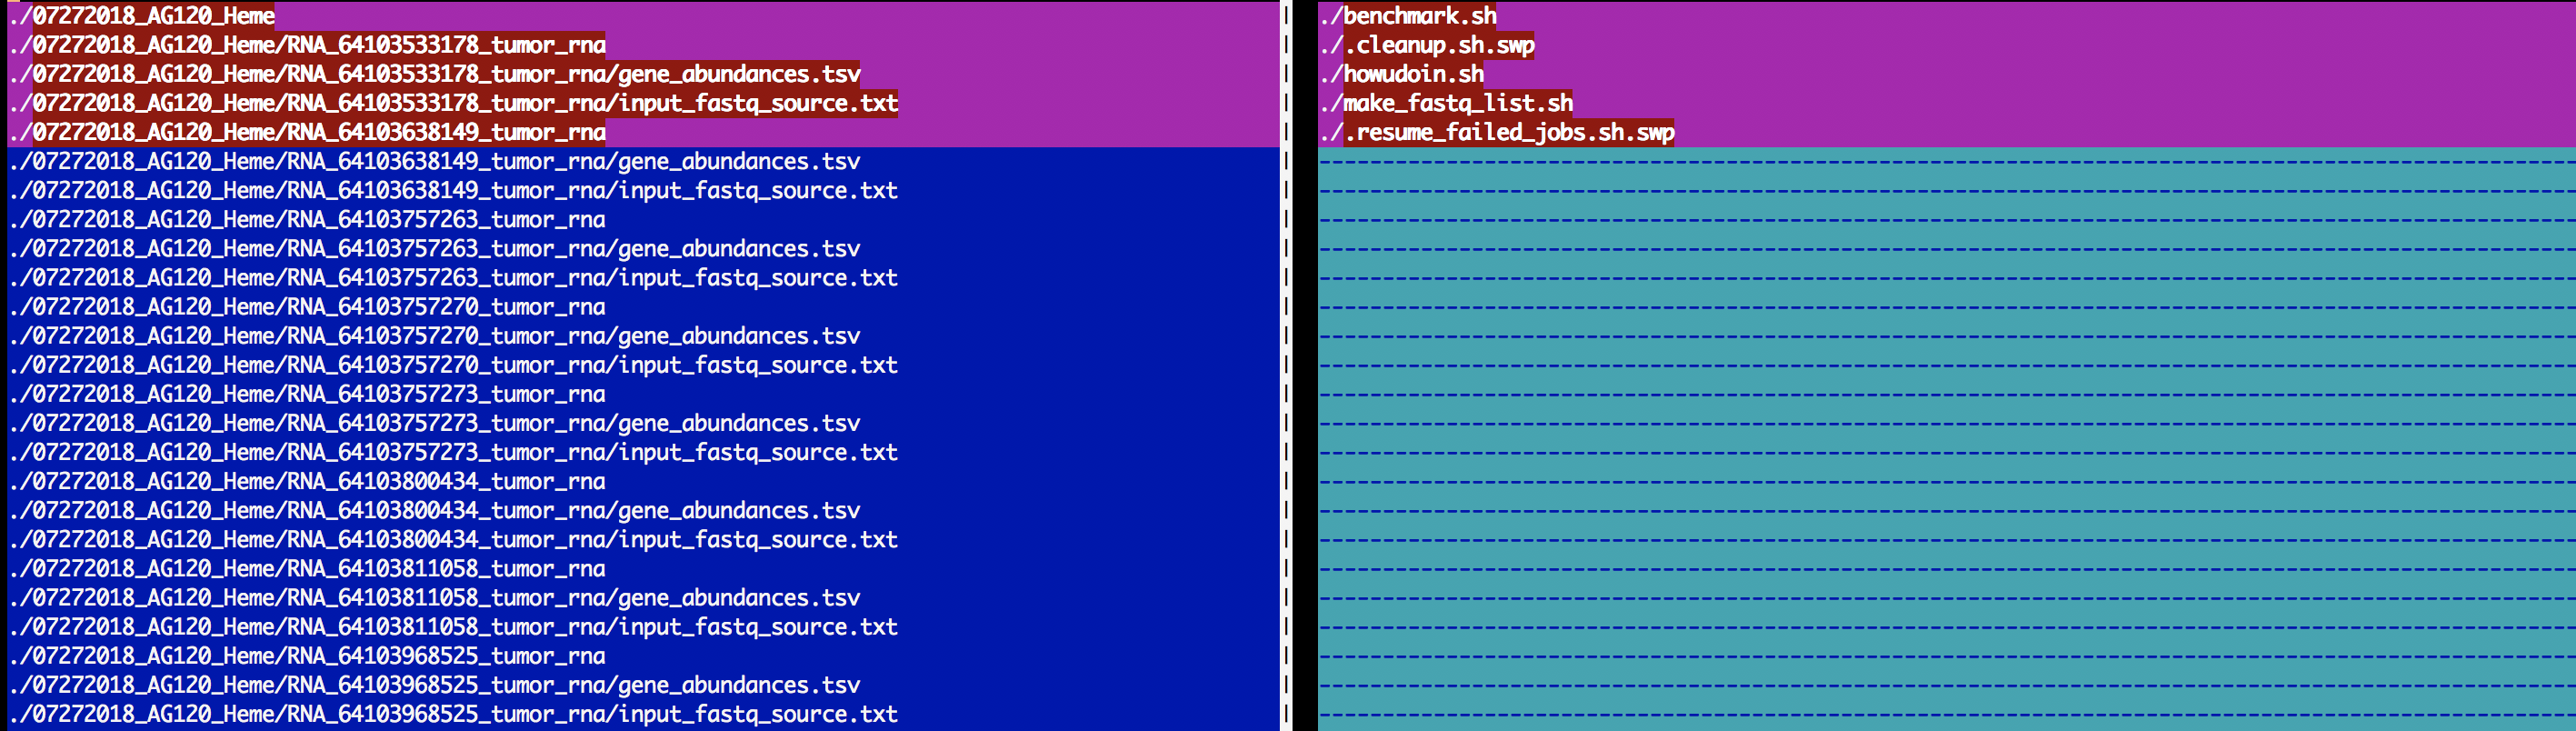
\includegraphics[width=1.3\linewidth]{images/vimdiff}

\hypertarget{sun-grid-engine}{%
\subsubsection{Sun Grid Engine}\label{sun-grid-engine}}

\hypertarget{deprioritize-jobs-queued-on-sge}{%
\paragraph{Deprioritize jobs queued on SGE}\label{deprioritize-jobs-queued-on-sge}}

\begin{Shaded}
\begin{Highlighting}[]
\NormalTok{qalter }\OperatorTok{-}\NormalTok{p }\DecValTok{-100}\NormalTok{ \{jobid1..jobidn\}}
\end{Highlighting}
\end{Shaded}

\hypertarget{vim}{%
\subsubsection{vim}\label{vim}}

\hypertarget{repeat-content-of-line-in-new-column}{%
\paragraph{Repeat content of line in new column}\label{repeat-content-of-line-in-new-column}}

\begin{verbatim}
# repeat content of line
# a
# b
# c
# becomes
# a = C.a
# b = C.b
# c = C.c
:%s/.*/& = C.&
\end{verbatim}

\hypertarget{r-1}{%
\subsection{R}\label{r-1}}

\hypertarget{heatmaps}{%
\subsubsection{Heatmaps}\label{heatmaps}}

\hypertarget{addition}{%
\subsubsection{Addition}\label{addition}}

\begin{Shaded}
\begin{Highlighting}[]
\NormalTok{x <-}\StringTok{ }\DecValTok{3}
\NormalTok{y <-}\StringTok{ }\DecValTok{4}
\NormalTok{z <-}\StringTok{ }\NormalTok{x }\OperatorTok{+}\StringTok{ }\NormalTok{y}
\NormalTok{z}
\end{Highlighting}
\end{Shaded}

\begin{verbatim}
## [1] 7
\end{verbatim}

\hypertarget{python}{%
\subsection{python}\label{python}}

\hypertarget{perl}{%
\subsection{perl}\label{perl}}

\hypertarget{get-number-of-lines-in-a-file}{%
\paragraph{Get number of lines in a file}\label{get-number-of-lines-in-a-file}}

\begin{Shaded}
\begin{Highlighting}[]
\FunctionTok{open}\NormalTok{(}\KeywordTok{my} \DataTypeTok{$input}\NormalTok{, }\KeywordTok{"}\StringTok{-|}\KeywordTok{"}\NormalTok{, }\KeywordTok{"}\StringTok{wc -l < }\DataTypeTok{$fastqs}\KeywordTok{"}\NormalTok{);}
\KeywordTok{my} \DataTypeTok{$rc}\NormalTok{ = <}\DataTypeTok{$input}\NormalTok{>;}
\KeywordTok{if}\NormalTok{ (}\DataTypeTok{$rc}\NormalTok{ =~ }\KeywordTok{/}\CharTok{(}\BaseNTok{\textbackslash{}d}\CharTok{+)}\KeywordTok{/}\NormalTok{) \{}
    \FunctionTok{print} \DataTypeTok{$rc}\NormalTok{;}
\NormalTok{\}}
\end{Highlighting}
\end{Shaded}

\bibliography{book.bib,packages.bib}


\end{document}
